\documentclass[12pt, letterpaper]{article}
\usepackage{silence}
\WarningFilter{latex}{Command \underbar has changed}
\WarningFilter{latex}{Command \underline has changed}

\usepackage[titletoc,title]{appendix}
\usepackage{color}
\usepackage{booktabs}
\usepackage[usenames,dvipsnames,svgnames,table]{xcolor}
\definecolor{dark-red}{rgb}{0.75,0.10,0.10}
\definecolor{bluish}{rgb}{0.05,0.05,0.85}

\usepackage[margin=1in]{geometry}
\usepackage[linkcolor=blue,
            colorlinks=true,
            urlcolor=blue,
            pdfstartview={XYZ null null 1.00},
            pdfpagemode=UseNone,
            citecolor={bluish},
            pdftitle={partisan gap}]{hyperref}

\usepackage[resetlabels,labeled]{multibib}
\newcites{SI}{SI References}
\usepackage{natbib}

\usepackage{float}

\usepackage{geometry}  % see geometry.pdf on how to lay out the page. There's lots.
\geometry{letterpaper} % This is 8.5x11 paper. Options are a4paper or a5paper or other...
\usepackage{graphicx}  % Handles inclusion of major graphics formats and allows use of
\usepackage{amsfonts,amssymb,amsbsy}
\usepackage{amsxtra}
\usepackage{verbatim}
\setcitestyle{round,semicolon,aysep={},yysep={;}}
\usepackage{setspace} % Permits line spacing control. Options are:
%\doublespacing
%\onehalfspace
\usepackage{sectsty}    % Permits control of section header styles
\usepackage{pdflscape}
\usepackage{fancyhdr}   % Permits header customization. See header section below.
\usepackage{url}        % Correctly formats URLs with the \url{} tag
\usepackage{fullpage}   %1-inch margins
\usepackage{multirow}
\usepackage{verbatim}
\usepackage{rotating}
\setlength{\parindent}{3em}

\usepackage[T1]{fontenc}

\usepackage{chngcntr}
\usepackage{longtable}
\usepackage{adjustbox}
\usepackage{dcolumn}

\usepackage[nameinlink, capitalize, noabbrev]{cleveref}

\def\citeapos#1{\citeauthor{#1}'s (\citeyear{#1})}

\makeatother

\usepackage{footmisc}
\setlength{\footnotesep}{\baselineskip}
\makeatother
\renewcommand{\footnotelayout}{\normalsize \doublespacing}


% Colors
\usepackage{color}

\newcommand{\bch}{\color{blue}\em  }   % begin change
\newcommand{\ying} {\color{orange}\em  }   % begin change
\newcommand{\bgcd} {\color{purple}\em }
\newcommand{\ech}{\color{black}\rm  }    % end change

% Caption
\usepackage[hang, font=small,skip=0pt, labelfont={bf}]{caption}
%\captionsetup[subtable]{font=small,skip=0pt}
\usepackage{subcaption}

% tt font issues
% \renewcommand*{\ttdefault}{qcr}
\renewcommand{\ttdefault}{pcr}


\setcounter{page}{0}

\usepackage{lscape}
\renewcommand{\textfraction}{0}
\renewcommand{\topfraction}{0.95}
\renewcommand{\bottomfraction}{0.95}
\renewcommand{\floatpagefraction}{0.40}
\setcounter{totalnumber}{5}
\makeatletter
\providecommand\phantomcaption{\caption@refstepcounter\@captype}
\makeatother

\title{A Measurement Gap? \\ 
       Effect of Survey Instrument and Scoring on the Partisan Knowledge Gap}
  
\author{Lucas Shen\thanks{Research Fellow, National University of Singapore, \href{lucas@lucasshen.com}{lucas@lucasshen.com}} 
\and
Gaurav Sood\thanks{Independent researcher, \href{gsood07@gmail.com}{gsood07@gmail.com}}  \and
Daniel Weitzel\thanks{Assistant Professor, Colorado State University, and Senior Research Fellow, University of Vienna, \href{mailto:daniel.weitzel@colostate.edu}{daniel.weitzel@colostate.edu}}}

\date{\today \thanks{Working paper, most recent version available at: \href{https://github.com/soodoku/partisan-gaps}{https://github.com/soodoku/partisan-gaps}}}

\begin{comment}

setwd(paste0(githubdir, "partisan-gaps/ms/"))
tools::texi2dvi("partisan_gap.tex", pdf = TRUE, clean = TRUE)
setwd(githubdir)

\end{comment}

% WORD COUNT 2023-10-15
% Just Text 5824
% References 1040
% tables and footnotes 1000
% total 8k


\begin{document}
\maketitle
\thispagestyle{empty}

\begin{abstract}

\noindent Research suggests that partisan gaps in political knowledge with partisan implications are wide and widespread. Using a series of experiments, we investigate the extent to which partisan gaps in commercial surveys are a result of differences in beliefs than motivated guessing. Knowledge items on commercial surveys often have features that encourage guessing. We find that removing such features yields scales with greater reliability and higher criterion validity. More substantively, partisan gaps on scales without these ``inflationary'' features are roughly 40\% smaller. Thus, contrary to \citet{prior2015you}, who find that the upward bias is explained by the knowledgeable deliberately marking the wrong answer (partisan cheerleading), our data suggest, in line with \citet{bullocketal_2015} and \citet{graham2023less}, that partisan gaps on commercial surveys are strongly upwardly biased by motivated guessing by the ignorant. Relatedly, we also find that partisans know less than what toplines of commercial polls suggest.
\end{abstract}

\vspace{.2in}

{\bf Keywords:} Political Knowledge; Partisan Gap; Motivated Skepticism

\newpage

\doublespacing

Wide and widespread partisan gaps challenge the idea that citizens can hold representatives accountable \citep{hochschild2015isn}. Hence, the alarm over research that suggests as much \citep{bartels_2002, campbell1980american, jerit2012partisan}. However, an emerging line of research argues that a large fraction of the partisan knowledge gap is an artifact of the survey response process \citep{bullocketal_2015, huber_yair_2018, prior2015you, graham2023less} (though see \citet{berinsky_2017}, \citet{peterson2021partisan}, and \citet{malka2022expressive}). In this paper, we extend this investigation.

Our starting point is commercial polls. In particular, we examine how common features of partisan knowledge items on commercial polls, e.g., presenting social proof about the less socially desirable option, not including a `Don't know' option, etc., affect partisan gaps in knowledge of facts with political implications. We find that removing guessing encouraging features yields knowledge scales with greater reliability and higher criterion validity. Substantively, we find that common design features of knowledge items on commercial polls are ``inflationary''---they dramatically inflate the actual partisan gap in beliefs. On average, these features artificially widen the partisan gap in beliefs by 40\% (14 percentage points). To further ablate response biases, we use an instrument and scoring scheme inspired by \citet{pasek2015} and \citet{graham2021measuring} that takes into account respondents' confidence in their answers. Using the scoring scheme that credits only confidently held beliefs as knowledge, we find that partisan gaps are another 50\% smaller.

Our results contribute to a growing literature that suggests that a large fraction of partisan gaps are artifacts of survey design. Our results also further clarify the source of bias in estimates of partisan gaps. While some previous research shows that the partisan gap is due to partisan cheerleading---deliberate picking of congenial incorrect answers by the knowledgeable \citep{prior2015you}, our data suggests that the bias in the estimate of the partisan gap is primarily a result of partisan guessing by the ignorant (see also \citet{bullocketal_2015} and \citet{graham2023less} who reach similar conclusions). 

Our results suggest that some concerns about democratic health are overstated and that some are underappreciated. Reducing guessing related error reveals that partisan gaps on partisan knowledge items are not as wide but also that partisans know less about politics than what the toplines of commercial polls suggest.

\section*{Theory, Motivation, and Empirical Strategy}\label{sec:theory}

``Has unemployment increased, decreased, or stayed the same since President Joe Biden took office in 2021?'' How knowledge about this fact and other such politically consequential facts is distributed across the population is relevant to the health of a democracy. If there are wide gaps in partisans' knowledge of politically relevant facts, citizens' ability to hold politicians accountable might be limited.

Concerningly, a large body of research finds that partisan gaps in political knowledge with partisan implications are both wide and widespread \citep{bartels_2002, jerit2012partisan, pew2018disagree, lodgetaber_2013} (though see \citet{roush2023}). Some recent research however shows that a large part of the partisan gaps stem from partisan responding rather than differences in what partisans know to be true about the world \citep{bullocketal_2015, prior2015you, huber_yair_2018, graham2023less} (though see \citet{peterson2021partisan}, \citet{berinsky_2017}, and \citet{malka2022expressive}). 

More generally, researchers argue that partisan gaps in political knowledge with partisan implications are inflated by: 

\begin{itemize}

    \item \textbf{Partisan Cheerleading.} Partisans who know the right uncongenial answer deliberately pick the wrong partisan congenial answer to register their support for their party or to influence the survey results \citep{prior2015you}.

    \item \textbf{Partisan Guessing.} Partisans who don't know the answer offer substantive responses congenial to their party \citep{bullocketal_2015, graham2023less}. For instance, when asked about what happened to the federal deficit during the Obama administration, Republicans, thinking Democrats cause bad things, may infer that deficits rose under Obama. And we expect Democrats to come to the opposite conclusion. We thus expect guessing-encouraging designs or designs that prime partisanship to increase partisan gaps.

\end{itemize}

In this paper, we interrogate the latter explanation in the context of commercial polls. An analysis of 180 media polls by \citet{luskinetal_nd} found that guessing encouraging features were exceedingly common. For instance, less than 9\% of the surveys offered an explicit `Don't Know' or `Not Sure' option, which causes a positive bias in the estimates of political knowledge \citep{luskin2011don}. And about half of the items offered only two choices, a design choice that dramatically inflates estimates of knowledge \citep{bullock2022response}. An overwhelming majority of the items (168) also included wording that encouraged guessing, by framing the factual question as one of a `matter of opinion.' They also found that the scoring rules used by analysts treated all correct responses--even when the respondent is unconfident about their answer---as evidence of knowledge. Doing so conflates guesses and on-the-spot inferences with knowledge \citep{pasek2015}. 

To study the effect of ``inflationary'' features of survey and question design on the partisan knowledge gap, we conduct a series of survey experiments that modify various guessing encouraging features. To study the effect of taking respondents' confidence in account, we draft an instrument and scoring rule inspired by \citet{pasek2015}, which uses self-assessed confidence to rescore the answers, taking only correct answers respondents are confident about as evidence that the respondent knows the fact. (Correct responses that respondents are confident about have higher test-retest reliability \citep{graham2021measuring} suggesting that these measures are also more valid.) Finally, we analyze which item formats yield more reliable measures of knowledge and have greater criterion validity. (We find that items without the ``inflationary'' features have higher criterion validity.)

In all, we use data from four surveys. The results of these four surveys are presented as part of three studies:

\begin{itemize}
    \item In Study 1, we use data from a survey experiment conducted on Amazon Mechanical Turk (MTurk) (\emph{MTurk 1}) to examine how guessing encouraging features affect the partisan gap. 
    \item In Study 2, we use survey experiments conducted on a \emph{YouGov} and a telephone survey (\emph{Texas Lyceum}) to examine the effect of partisan cues on the partisan gap.
    \item Lastly, in Study 3, we use data from \emph{MTurk 1} and another survey fielded on MTurk (\emph{MTurk 2}) to study the impact of taking respondents' confidence in their answers on the partisan gap.
\end{itemize}

Before we proceed further, we would like to note that many of our questions are on topics on which people can be misinformed---know the wrong thing confidently. This includes partisan retrospection items like those used by \cite{bartels_2002}. However, on all of these `misinformation' items, we can also ask how many people know the right answer. Like \citet{bartels_2002} and \citet{prior2015you}--- and for much the same reasons--- we are interested in measuring the partisan gap in knowledge, though we believe that it would be useful to study partisan gaps in misinformation. 

\section*{Study 1: The Effect of Guessing Encouraging Features} \label{sec:inflationary_measures}

The first study focuses on three survey design features that we suspect inflate the partisan gap. These features are: 

\begin{enumerate}
    \item the absence of a ``Don't Know'' option,
    \item including additional neutral or partisan information in the question stem, and
    \item the absence of a guessing discouraging preamble.
\end{enumerate}

\subsection*{Research Design and Data}\label{subsec:data1}

We conducted a survey experiment on MTurk in mid-2017 in which we randomly assigned 1,253 respondents to one of four conditions (see Table \ref{tab:conditions} for a summary.)\footnote{For generalizability of effects in studies conducted on MTurk, see \citep{mullinix2015generalizability, coppock2018generalizability}.} In each condition, respondents answered nine misinformation items, ranging from President Obama's citizenship to whether global warming is happening or not. (For exact question wording for each of the items, see \cref{si:mturk1}.)

The four conditions are:

\begin{description}

    \item[Inflationary Design Approach (IDA)] \phantomsection\label{txt:IDA} The IDA serves as our baseline condition. The items in this condition include all the common features of commercial polls. In this design, the `Don't Know' option is never presented, so respondents cannot indicate that they don't know the answer. The questions also include social proof about the incorrect answer. For instance, on a question about where Mr. Obama was born, we add ``some people believe Barack Obama was not born in the United States but was born in another country.'' In other cases, we provide some neutral information about the topic, like ``According to the Constitution, American presidents must be natural-born citizens.'' Lastly, the preamble to the knowledge questions is neutral and doesn't discourage guessing or cheating. The preamble simply reads: ``Now here are some questions about what you may know about politics and public affairs...''
    
    \item[Commonly Used Design (CUD)] \phantomsection\label{txt:CUD} CUD makes one change to the IDA. Like the IDA, the questions do not feature a `Don't Know' option and include neutral information in the question stem that encourages guessing. However, the questions do not include social proof.

    \item[Fewer Substantive Responses (FSR)] \phantomsection\label{txt:FSR} FSR makes two changes to CUD. First, the preamble discourages blind guessing and cheating. The preamble reassures respondents that it is okay not to know the answers to these questions, asks respondents to commit to not look up answers or ask anyone, and asks respondents to mark don't know when they don't know the answer. Second, the items now include a `Don't Know' option \citep[see, e.g.,][]{luskin2011don, bullocketal_2015}.

    \item[Improved Multiple Choice (IMC)] \phantomsection\label{txt:IMC} IMC is the best version of these multiple choice questions. It offers respondents a `Don't Know' option and does not include guessing encouraging neutral information or social proof.
\end{description}

\begin{table}[H]
\centering
\caption{Experimental Treatments}
\label{tab:conditions}
\begin{tabular}{ccccccc}
\hline
           & \multicolumn{6}{c}{\textbf{Treatments}}              \\
 Condition & Label & Don't & Social & Guessing   & Neutral     & Confidence \\
           &       & Know  & Proof  & Encouraged & Information & Coding  \\ \hline
 1        & \hyperref[txt:IDA]{IDA} & No    & Yes    & Yes        &  Yes        & No         \\
 2        & \hyperref[txt:CUD]{CUD} & No    & No     & Yes        &  Yes        & No         \\
 3        & \hyperref[txt:FSR]{FSR} & Yes   & No     & No         &  Yes        & No         \\
 4        & \hyperref[txt:IMC]{IMC}& Yes   & No     & No         &  No         & No         \\
% 5        & \hyperref[txt:CCD]{CCD} & No    & No     & No         &  No         & Yes        \\
  \hline
\end{tabular}
\end{table}
{}

\subsection*{Measures}\label{subsec:study1_measures}
We measure partisanship using the conventional branched seven-point partisan self-identification scale. Independents who lean toward one of the two major parties are coded as supporters of that party. A knowledge item is coded as congenial if the correct answer is congenial to the partisanship of the respondent.

\subsection*{Results}\label{subsec:study1_results}

We start by summarizing the average partisan gap on each survey item in each treatment arm (see \Cref{fig:partisangaps-mturk}).\footnote{Balance tests suggest that the randomization was successful (see \crefrange{fig:baltest-RW-ips}{fig:baltest-24k-ips}).} In the baseline IDA condition (first column), when the correct response is congenial to the respondents' party, respondents are 35 percentage points more likely to choose the correct response. The partisan gap is unresponsive to the changes made in CUD. However, the estimates from the FSR and IMC conditions are approximately 14 percentage points lower than in the IDA. The 14 percentage points reduction translates to a 40\% relative drop ($100 \times \frac{.35-.21}{.35}$). 

% Table for the unstandardized partisan gap estimates from study 1

% results are presented in the partisan-gap-by-item-arm.pdf figure

%\begin{table}[t] \centering \scriptsize \setlength\tabcolsep{0 pt} \setlength{\defaultaddspace}{0pt}
\caption{Unstandardized Partisan Gaps in Knowledge}
\label{tab:partisangaps-mturk}	
	\begin{adjustbox}{max width=\textwidth}
		\begin{tabular}{l*{15}{D{.}{.}{-1}}}	
			\toprule  
			& \multicolumn{3}{c}{RW} & \multicolumn{3}{c}{IPS} & \multicolumn{3}{c}{FSR} & \multicolumn{3}{c}{14k} & \multicolumn{3}{c}{24k} \\
			\cmidrule(lr){2-4} \cmidrule(r){5-7} \cmidrule(r){8-10} \cmidrule(r){11-13} \cmidrule(){14-16}                
			            & \multicolumn{1}{c}{Dem.}   & \multicolumn{1}{c}{Rep.} & \multicolumn{1}{c}{Gap} & \multicolumn{1}{c}{Dem.}   & \multicolumn{1}{c}{Rep.} & \multicolumn{1}{c}{Gap} & \multicolumn{1}{c}{Dem.}   & \multicolumn{1}{c}{Rep.} & \multicolumn{1}{c}{Gap} & \multicolumn{1}{c}{Dem.}   & \multicolumn{1}{c}{Rep.} & \multicolumn{1}{c}{Gap} & \multicolumn{1}{c}{Dem.}   & \multicolumn{1}{c}{Rep.} & \multicolumn{1}{c}{Gap} \\
			\cmidrule(lr){2-4} \cmidrule(lr){5-7} \cmidrule(lr){8-10} \cmidrule(lr){11-13} \cmidrule(l){14-16}    
			Obama birthplace    & 0.01       & 0.45       & 0.443    & 0.03       & 0.36       & 0.328    & 0.03       & 0.16       & 0.127    & 0.06       & 0.15       & 0.086      & 0.03       & 0.2        & 0.174    \\
			& {[}0.01{]} & {[}0.07{]} & {[}0.052{]} & {[}0.02{]} & {[}0.07{]} & {[}0.056{]} & {[}0.02{]} & {[}0.05{]} & {[}0.042{]} & {[}0.02{]} & {[}0.05{]} & {[}0.049{]} & {[}0.01{]} & {[}0.06{]} & {[}0.045{]} \\
			Obama religion      & 0.11       & 0.7        & 0.586    & 0.09       & 0.5        & 0.415    & 0.1        & 0.39       & 0.291    & 0.13       & 0.3        & 0.164     & 0.02       & 0.19       & 0.171    \\
			& {[}0.03{]} & {[}0.06{]} & {[}0.064{]} & {[}0.03{]} & {[}0.07{]} & {[}0.065{]} & {[}0.03{]} & {[}0.07{]} & {[}0.061{]} & {[}0.03{]} & {[}0.07{]} & {[}0.066{]} & {[}0.01{]} & {[}0.07{]} & {[}0.044{]} \\
			ACA illegal         & 0.21       & 0.68       & 0.465    & 0.17       & 0.66       & 0.490    & 0.1        & 0.34       & 0.238    & 0.17       & 0.43       & 0.256    & 0          & 0.15       & 0.147    \\
			& {[}0.04{]} & {[}0.06{]} & {[}0.074{]} & {[}0.04{]} & {[}0.07{]} & {[}0.073{]} & {[}0.03{]} & {[}0.06{]} & {[}0.060{]} & {[}0.04{]} & {[}0.07{]} & {[}0.072{]} & {[}0.00{]} & {[}0.06{]} & {[}0.044{]} \\
			ACA death panels    & 0.24       & 0.45       & 0.208    & 0.15       & 0.42       & 0.271    & 0.08       & 0.25       & 0.165    & 0.09       & 0.32       & 0.230    & 0.13       & 0.13       & 0.007       \\
			& {[}0.04{]} & {[}0.07{]} & {[}0.078{]} & {[}0.04{]} & {[}0.07{]} & {[}0.072{]} & {[}0.03{]} & {[}0.06{]} & {[}0.055{]} & {[}0.03{]} & {[}0.07{]} & {[}0.061{]} & {[}0.04{]} & {[}0.06{]} & {[}0.074{]} \\
			GW causes           & 0.09       & 0.66       & 0.569    & 0.06       & 0.62       & 0.556    & 0.13       & 0.48       & 0.355    & 0.06       & 0.57       & 0.512    & 0.01       & 0.26       & 0.248    \\
			& {[}0.03{]} & {[}0.07{]} & {[}0.063{]} & {[}0.03{]} & {[}0.07{]} & {[}0.061{]} & {[}0.03{]} & {[}0.07{]} & {[}0.064{]} & {[}0.02{]} & {[}0.07{]} & {[}0.059{]} & {[}0.01{]} & {[}0.07{]} & {[}0.043{]} \\
			GW scientists agree & 0.03       & 0.34       & 0.309    & 0.1        & 0.32       & 0.224    & 0.06       & 0.23       & 0.173    & 0.09       & 0.32       & 0.230    & 0.03       & 0.02       & -0.004      \\
			& {[}0.02{]} & {[}0.07{]} & {[}0.054{]} & {[}0.03{]} & {[}0.07{]} & {[}0.064{]} & {[}0.02{]} & {[}0.06{]} & {[}0.050{]} & {[}0.03{]} & {[}0.07{]} & {[}0.061{]} & {[}0.02{]} & {[}0.02{]} & {[}0.028{]} \\
			Voter fraud         & 0.16       & 0.66       & 0.497    & 0.12       & 0.8        & 0.683    & 0.14       & 0.36       & 0.213    & 0.1        & 0.26       & 0.157    & 0.04       & 0.18       & 0.142    \\
			& {[}0.04{]} & {[}0.07{]} & {[}0.070{]} & {[}0.03{]} & {[}0.06{]} & {[}0.062{]} & {[}0.03{]} & {[}0.06{]} & {[}0.065{]} & {[}0.03{]} & {[}0.06{]} & {[}0.060{]} & {[}0.02{]} & {[}0.06{]} & {[}0.046{]} \\
			MMR vaccine         & 0.12       & 0.17       & 0.047       & 0.05       & 0.2        & 0.147    & 0.06       & 0.16       & 0.101     & 0.05       & 0.15       & 0.095     & 0.01       & 0.02       & 0.014       \\
			& {[}0.03{]} & {[}0.05{]} & {[}0.059{]} & {[}0.02{]} & {[}0.06{]} & {[}0.052{]} & {[}0.02{]} & {[}0.05{]} & {[}0.047{]} & {[}0.02{]} & {[}0.05{]} & {[}0.047{]} & {[}0.01{]} & {[}0.02{]} & {[}0.021{]} \\
			Budget deficit      & 0.67       & 0.92       & 0.251    & 0.89       & 0.94       & 0.046       & 0.95       & 0.89       & -0.056      & 0.7        & 0.94       & 0.240    & 0.85       & 0.92       & 0.073       \\
			& {[}0.05{]} & {[}0.04{]} & {[}0.070{]} & {[}0.03{]} & {[}0.03{]} & {[}0.050{]} & {[}0.02{]} & {[}0.04{]} & {[}0.041{]} & {[}0.04{]} & {[}0.04{]} & {[}0.071{]} & {[}0.04{]} & {[}0.04{]} & {[}0.065{]} \\
			Average             & 0.12       & 0.49       & 0.375    & 0.09       & 0.44       & 0.347    & 0.08       & 0.29       & 0.207    & 0.09       & 0.32       & 0.225    & 0.03       & 0.13       & 0.099    \\
			& {[}0.02{]} & {[}0.03{]} & {[}0.030{]} & {[}0.02{]} & {[}0.04{]} & {[}0.036{]} & {[}0.02{]} & {[}0.03{]} & {[}0.032{]} & {[}0.02{]} & {[}0.03{]} & {[}0.033{]} & {[}0.01{]} & {[}0.03{]} & {[}0.025{]}\\
			\bottomrule                    
		\end{tabular}
	\end{adjustbox}
\caption*{\scriptsize Difference in partisan gaps in knowledge (Republican - Democrats) for each of the nine questions in the MTurk sample and for the average difference in knowledge gap over all nine questions. Standard errors in brackets.}
\end{table}

% partisan-gaps/scripts/Stata/mturk/fig-partisan-gap.do
 
\begin{figure}[ht]
        \centering
        \caption{Partisan Gap by Treatment Arm (MTurk 1)}
        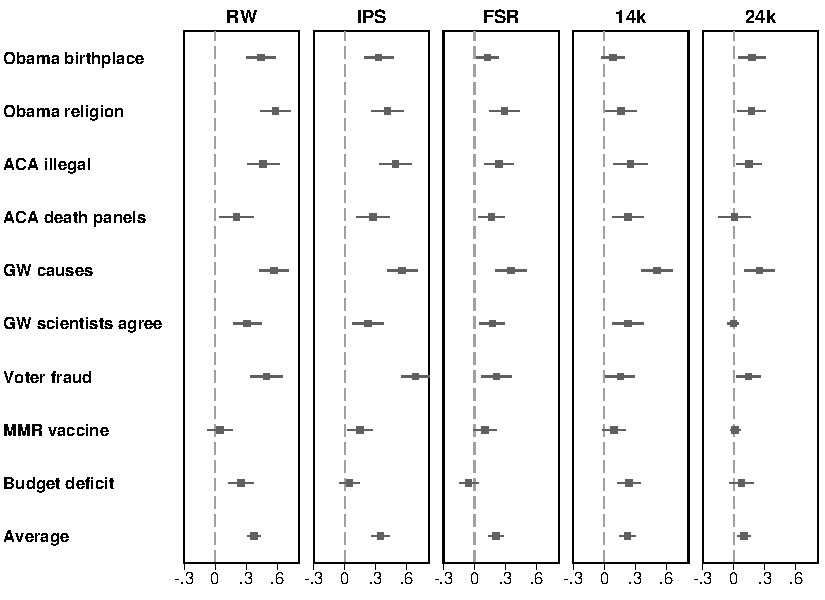
\includegraphics[width=\textwidth]{../figs/partisan-gap-by-item-arm.pdf}
        \label{fig:partisangaps-mturk}
        \caption*{\footnotesize The figure shows the estimated partisan gap in each of the nine knowledge items (see \cref{si:mturk1} for the details of the items) and the average partisan gap across the four conditions \Cref{tab:conditions}. The partisan gap is estimated using the linear model $\text{Correct response}_{i} = \alpha + \beta \text{congenial}_i + \varepsilon_i$ where `congenial' is a dummy variable that takes the value 1 when the correct response is congenial to the party. Horizontal bars are 95\% confidence intervals constructed from robust standard errors.}
\end{figure}

To formally test our hypothesis, we regress whether the answer is correct, on the interaction of the survey conditions and the congenial dummy. For respondent $i$, survey item $j$, and condition $k$, we estimate the following equation:

\begin{equation}\label{eq:partisangap-mturk} 
\text{Correct}_{ijk} = \alpha + \beta \text{Congenial}_i + \gamma \text{Condition}_k +  \delta_k (\text{Congenial}_i \times \text{Condition}_k) + \text{question}_j + \varepsilon_{ijk}
\end{equation}

$\beta$ captures the difference in the proportion of correct responses when the answer is congenial to the respondent's party. The $\delta_k$s capture how the three conditions (CUD, FSR, IMC) affect the partisan knowledge gaps vs. the baseline condition (IDA). We include item fixed-effects and cluster standard errors by respondent.

% partisan-gaps/scripts/Stata/mturk/reg-table.do
\begin{table}[t] \centering \small \setlength\tabcolsep{0 pt} \setlength{\defaultaddspace}{0pt}
    \def\sym#1{\ifmmode^{#1}\else\(^{#1}\)\fi}
    \caption{The Effect of Various Treatments on the Partisan Gap (MTurk 1)}
    \label{tab:partisangaps-mturk}
    \begin{adjustbox}{max width=\textwidth}
        \begin{tabular}{l*{6}{D{.}{.}{-1}}}
            \toprule
            \input ../tabs/mturk-reg-table-fragment.tex
            \bottomrule
        \end{tabular}
    \end{adjustbox}
    \caption*{\footnotesize All models are linear probability models where the dependent variable is whether the response is correct or not. See \cref{tab:conditions} for the description of the IDA, CUD, FSR, and IMC conditions. Demographic controls include age, gender, education, and race. Standard errors are clustered at the respondent level. Significance levels: + 0.1 * 0.05 ** 0.01 *** 0.001.}
\end{table}

\cref{tab:partisangaps-mturk} reports the results. Column (1) includes just the congenial variable, which is significant and consistent with conventional wisdom about gaps in partisan knowledge \citep[e.g.][]{bullocketal_2015, pew2018disagree}.

Column (2) only includes the survey conditions. The sharp negative coefficients on FSR and IMC show that respondents' estimated knowledge is sharply lower in the two conditions compared to the baseline. In column (3), we include the interaction between congenial and the three conditions (baseline is IDA). Now, the congenial variable captures the knowledge gap in the IDA condition (corresponding to column (1) of \cref{fig:partisangaps-mturk}). The congenial and survey condition interactions reveal the extent to which partisan knowledge gaps change across the different survey conditions. 

Columns (4)--(6) of \cref{tab:partisangaps-mturk} show that including self-reported characteristics of respondents does not change the conclusion. Overall, Study 1 suggests that partisan gaps are much larger in surveys that feature guessing encouraging features like the absence of a 'Don't Know' option, fewer response options, etc., which are common in commercial polls.

\section*{Study 2: The Effect of Partisan Cues on Partisan Gaps}\label{sec:partisan_cues}

In Study 2, we investigate the impact of partisan priming. We test it by manipulating whether the question stem has a partisan cue or not. We expect the presence of a partisan cue to exacerbate partisan gaps \citep{prior2015you}. 

\subsection*{Research Design and Data}\label{subsec:data2}

To answer the question, we leverage data from two surveys: a national survey conducted by YouGov (Study 2), and a telephone survey in Texas (Study 3). The YouGov survey includes data from 2,000 respondents who were interviewed between July 10th and 12th, 2012. The Texas survey has data from 1,003 respondents who were interviewed between September 10th and 21st, 2012.

In the YouGov survey, we asked respondents two retrospective economic evaluation questions: unemployment and the budget deficit. To manipulate congeniality, we randomly inserted a Republican or a Democratic cue into the question stem. In particular, we asked the following two questions:

\begin{enumerate}
\item Since the 2010 midterm elections, (``when Republicans regained control of the U.S. Congress'' or ``when Democrats retained control of the Senate'') the unemployment rate [had] gone up, down, or remained the same, or couldn't you say? 
\item Since the 2010 midterm elections, (``when Republicans regained control of the U.S. Congress" or ``when Democrats retained control of the Senate''), has the budget deficit gone up, gone down, remained the same, or couldn't you say?
\end{enumerate}

In the Texas survey, we added a `no partisan cue' condition to the unemployment rate question. A third of the respondents saw our third option: 

\begin{enumerate}\addtocounter{enumi}{+2}
    \item Since the 2010 midterm elections has the unemployment rate gone up, gone down, or remained the same? Or couldn't you say?
\end{enumerate}

We made two more changes to the second and final question on the Texas survey. First, we switched the question from one about budget deficits to one about federal tax rates. Second, we changed the treatment conditions to 1. no partisan cue, 2. Democratic cue, and 3. Democratic cue with a substantive response encouraging phrase. Respondents assigned to `no partisan cue' saw ``Since January 2009, have federal taxes increased, decreased, or remained the same, or couldn't you say?.'' The Democratic cue condition prepended ``Since Barack Obama took office\ldots'' to the question. The last version prepended a substantive response encouraging phrase. The question now read: ``Based on what you have heard, since Barack Obama took office, \ldots''

\subsection*{Study 2: YouGov Results}\label{subsec:yougov_results}

We estimate the impact of partisan cues by regressing whether the response is correct or not on the partisan congeniality of the cue. We code the cue as congenial if it increases the probability that the respondent would get the right correct by using partisan reasoning. For instance, if the right answer is that the objective conditions over some time period became worse, then highlighting that the opposing party controlled Congress during that time would be a congenial cue.

\begin{equation}\label{eq:pgap-yougov}
\text{Correct}_{i} = \alpha + \beta (Congenial \; Cue)_i  +\varepsilon_{i},
\end{equation}

% partisan-gaps/scripts/Stata/survey-exp/reg-table.do
\begin{table}[t] \centering \normalsize \setlength\tabcolsep{0 pt} \setlength{\defaultaddspace}{0pt}
    \def\sym#1{\ifmmode^{#1}\else\(^{#1}\)\fi}
    \caption{The Impact of Partisan Cues on Partisan Gaps (YouGov)}
    \label{tab:partisangaps-yougov}
    \begin{adjustbox}{max width=\textwidth}
        \begin{tabular}{@{\hspace{0\tabcolsep}}l*{6}{D{.}{.}{-1}}@{\hspace{0\tabcolsep}}}
            \toprule
            % https://tex.stackexchange.com/questions/567985/problems-with-inputtable-tex-hline-after-2020-fall-latex-release
            &\multicolumn{2}{c}{Unemployment has gone up}&\multicolumn{2}{c}{Deficit has gone up}\\
            \cmidrule(lr){2-3}\cmidrule(l){4-5} 
            \input ../tabs/yougov-reg-table-fragment.tex
            \bottomrule
        \end{tabular}
    \end{adjustbox}
    \caption*{\footnotesize Dependent variables indicate whether or not the respondent chose the correct answer. Demographic controls include age cohort, gender, education level, marital status, employment status, news interest, family income, and race. Standard errors are heteroskedasticity-robust. 
        All models are linear probability models. 
        Significance levels: + 0.1 * 0.05 ** 0.01 *** 0.001.}
\end{table}

% partisan-gaps/scripts/Stata/survey-exp/unemp-barplots.do
% partisan-gaps/scripts/Stata/survey-exp/deficit-barplots.do

\begin{figure}[t]
    \caption{Partisan Gap by Treatment Arm (YouGov)}    
    \centering
    \begin{subfigure}{.495\textwidth}\centering
        \includegraphics[width=\textwidth]{../figs/yougov-unemp-congenialcue.pdf}
        \caption{Unemployment}
    \end{subfigure}
    \hfil
    \begin{subfigure}{.495\textwidth}\centering
        \includegraphics[width=\textwidth]{../figs/yougov-deficit-congenialcue.pdf}
        \caption{Budget deficit}
    \end{subfigure} 
    \caption*{\footnotesize Bars indicate the predicted percent of correct answers as reported in \cref{tab:partisangaps-yougov} (columns (1) and (4)).  
        Capped vertical bars indicate 95\% confidence intervals.
    }
    \label{fig:yougov-reg}
\end{figure}

\cref{fig:yougov-reg} plots the results. As Panel (a) of \cref{fig:yougov-reg} illustrates, showing a congenial cue instead of an uncongenial one causes the probability of the correct response on the unemployment question to increase by 14 percentage points ($p < 0.001$, reported in \cref{tab:partisangaps-yougov}). Panel (b) of \cref{fig:yougov-reg} shows that this effect is not unique to the unemployment question. On the budget deficit question, the difference is 18 percentage points ($p<0.001$). Partisans are therefore more likely to respond correctly to a survey question when there is a partisan cue in the question stem that frames the right answer as congenial to the party.

\subsection*{Study 2: Texas Lyceum Results}\label{subsec:txlyceum_results}

% partisan-gaps/scripts/Stata/tx-lyceum/unemp-barplot.do
\begin{figure}[!t]
    \centering
    \caption{Partisan Gap on Unemployment by Treatment Arm (Texas Lyceum)}
    \includegraphics[width=.55\textwidth]{../figs/texas-unemp-congenialcue.pdf}
    \label{fig:partisangaps-texas-unemp}
    \caption*{\footnotesize 
        Bars indicate the predicted percent of responses saying that unemployment has gone up (correct response) as reported in column (1) of \cref{tab:partisangaps-texas-unemp}.  
        Capped vertical bars indicate 95\% confidence intervals.
    }
\end{figure}

We supplement our results with the Texas Lyceum survey. As \cref{fig:partisangaps-texas-unemp} shows, on the unemployment question, the pattern we saw on YouGov still holds when we include a neutral cue. Compared to respondents who received a neutral cue, respondents who received an uncongenial cue were 17 percentage points less likely to get the correct answer ($p<0.001$). While respondents who received a congenial cue were 8 percentage points more likely to get the correct answer ($p<0.1$). These results are tabulated in \cref{tab:partisangaps-texas-unemp}.

% partisan-gaps/scripts/Stata/tx-lyceum/reg-table.do
\begin{table}[t] \centering \normalsize \setlength\tabcolsep{6 pt} \setlength{\defaultaddspace}{0pt}
    \def\sym#1{\ifmmode^{#1}\else\(^{#1}\)\fi}
    \caption{Partisan Gap on Unemployment by Treatment Arm (Texas Lyceum)}
    \label{tab:partisangaps-texas-unemp}
    \begin{adjustbox}{max width=\textwidth}
        \begin{tabular}{@{\hspace{0\tabcolsep}}l*{3}{D{.}{.}{-1}}@{\hspace{0\tabcolsep}}}
            \toprule
            % https://tex.stackexchange.com/questions/567985/problems-with-inputtable-tex-hline-after-2020-fall-latex-release
            &\multicolumn{3}{c}{Unemployment has gone up}\\
            \cmidrule(l){2-4}
            \input ../tabs/texas-unemp-reg-table-fragment.tex
            \bottomrule
        \end{tabular}
    \end{adjustbox}
    \caption*{\footnotesize The Dependent variable is whether or not the respondent got the answer correct.  
        Demographic controls include age cohort, gender, education level, marital status, number of children, children's school enrollment, family income, religion, liberalism/conservatism, and race. Standard errors are heteroskedasticity-robust. 
        All models are linear probability models. 
        Significance levels: + 0.1 * 0.05 ** 0.01 *** 0.001.}
\end{table}

% partisan-gaps/scripts/Stata/tx-lyceum/reg-table.do
\begin{table}[t] \centering \normalsize \setlength\tabcolsep{6 pt} \setlength{\defaultaddspace}{0pt}
    \def\sym#1{\ifmmode^{#1}\else\(^{#1}\)\fi}
    \caption{Impact of Various Treatments on Partisan Gap on Federal Taxes (Texas Lyceum)}
    \label{tab:partisangaps-texas-fedtax}
    \begin{adjustbox}{max width=\textwidth}
        \begin{tabular}{@{\hspace{0\tabcolsep}}l*{4}{D{.}{.}{-1}}@{\hspace{0\tabcolsep}}}
            \toprule
            % https://tex.stackexchange.com/questions/567985/problems-with-inputtable-tex-hline-after-2020-fall-latex-release
            &\multicolumn{2}{c}{Responded ``Gone up''}&\multicolumn{2}{c}{Responded ``Don't Know''}\\
            \cmidrule(lr){2-3}\cmidrule(l){4-5} 
            \input ../tabs/texas-fedtax-reg-table-fragment.tex
            \bottomrule
        \end{tabular}
    \end{adjustbox}
    \caption*{\footnotesize The dependent variable is whether or not the respondent got the answer correct. Demographic controls include age cohort, gender, education level, marital status, number of children, children's school enrollment, family income, religion, liberalism/conservatism, and race. Standard errors are heteroskedasticity-robust. 
        All models are linear probability models. 
        Significance levels: + 0.1 * 0.05 ** 0.01 *** 0.001.}
\end{table}

Finally, we examine the federal tax rate question in the Texas Lyceum survey. As \cref{tab:partisangaps-texas-fedtax} shows, randomly receiving a congenial cue leads to a 21.5 percentage points increase in the chance of getting the answer right compared to the neutral cue condition ($p<0.001$). On the other hand, an uncongenial cue leads to a 29.8 percent lower chance ($p<0.001$). We also estimate how the cue that encourages guessing affects the ``Don't Know'' response rate. Including a substantive response encouraging cue does not have a stark effect. Overall, results from Studies 2 and 3 show that partisan cues dramatically affect the size of partisan gaps. If partisan gaps only reflected partisans' existing stores of knowledge, the gaps would be unresponsive to these cues. Thus, the data show that the partisan gap in the presence of partisan cues is upwardly biased.    

\section*{Study 3: The Effect of the Scoring Method on Partisan Gaps} \label{sec:confidence_coding}

Lastly, we examine the consequences of scoring decisions on partisan gaps. We introduce an assessment that takes into account respondents' confidence in their answers. Our goal here is to only score true political knowledge, the confidently held correct beliefs about political facts. 

\subsection*{Research Design and Data}\label{sec:data3}

Knowledge questions are commonly offered as multiple-choice items and conventionally, if a respondent marks the right answer, it is taken as evidence that the respondent truly knows the answer. Such scoring does not differentiate between confidently held beliefs, hunches, inferences, blind guesses, and expressive responses. To distinguish between hunches, guesses, and confidently held beliefs, we use the design from studies like \citet{pasek2015}. In our Confidence Coding Design (CCD) respondents rate claims on a Likert scale going from `definitely false' (0) to `definitely true' (10). 

To estimate the impact of the question and scoring design that takes respondents' confidence in their answers into account, we use data from two separate surveys. Our first survey is the one underlying Study 1 (\emph{MTurk 1}). The survey had a fifth condition in addition to the four conditions presented above. The fifth condition offered the same questions, except this time respondents were asked to respond on a Likert scale ranging from 0 (definitely not true) to 10 (definitely true). The CCD condition builds on the first four conditions and does not encourage guessing and features no social proof. (The question wording for the items is presented in \cref{si:mturk1}.) Since the items are dichotomous choice, the CCD scoring is straightforward. We scored respondents who marked `definitely true' about the right answer as knowledgeable.\footnote{In \cref{si_alternate_coding}, we try less stringent criteria and the main picture remains broadly unchanged.}

For the second study, we turn to another MTurk survey (\emph{MTurk 2}). In the survey, we randomly assigned 1,059 respondents to two conditions. The preamble, topics, and answer options of these questions were identical to the first survey and included questions about the Affordable Care Act (2), the effect of greenhouse gases (1), and the consequences of Mr. Trump's executive order on immigration (1). In the multiple-choice version of the item, participants received three options. In two of the four conditions, respondents also had a ``Don't Know'' option available to them. (For question text, see \cref{si:mturk2}.)

The scoring for this study is more nuanced, as the multiple-choice questions had four potential response options. In the CCD treatment, survey participants see the same question as in the multiple choice treatment, but have to rank the correctness of all the \emph{n} answer options from the multiple choice treatment. Broadly, we code an answer as correct if the respondent indicates that they are confident that the correct answer is correct and when they do not indicate that any of the incorrect options might also be correct. But more precisely, we code a response as correct if four conditions are met:

\begin{enumerate}

  \item The respondent is most confident about the correct answer. For instance, it shouldn't be the case that the respondent is more confident about an incorrect answer.

  \item The respondent cannot be as confident about the correct answer as any other option. For instance, it cannot be that the four options are all rated 10. 

  \item The respondent must be at least $\beta$ confident in the correct answer. In the main text, we use a $\beta$ of 10 but in \cref{si_alternate_coding}, we try less stringent criteria.

  \item The confidence in the incorrect answers cannot be above $\theta$. In the main text, we use a $\theta$ of 0 but in the \cref{si_alternate_coding}, we try less stringent criteria.

\end{enumerate}

\subsection*{Study 3: MTurk 1 Results}

The best version of the dichotomous multiple-choice items (IMC) showed a partisan gap of .22 (see \cref{fig:partisangaps-mturk}). As \cref{fig:mturk_hk24} shows, nearly half of the gap vanishes under the confidence scoring of CCD. Furthermore, the number of items where there is no statistically significant gap between partisans doubles from two to four. In all, there is a nearly 11 percentage point drop in the size of the partisan gap when we treat only confident correct answers as evidence that the respondent knows the answer. 

\begin{center}
    \begin{figure}[ht]
        \centering
        \caption{Partisan Gaps in Knowledge in Different Question Designs}
        \includegraphics[width=.9\textwidth]{../figs/partisan-gap-by-item-arm-14k-24k.pdf}
        \label{fig:mturk_hk24}
        \caption*{\footnotesize
            The figure shows the estimated partisan gaps in knowledge from MTurk 1 for two different survey conditions. The CCD condition only considers selecting the right answer with complete confidence as evidence that the respondent knows the answer (see \cref{si:mturk2}).
            See \crefrange{tab:confidence-scoring-study1}{tab:confidence-scoring-study1-ccd-14k-imc} in \cref{si:mturk1-ccd} for the regression estimates of the multiple-choice conditions to the confidence coding condition.
            See \cref{fig:mturk_hk24_mc} for the same analysis with all four multiple-choice conditions pooled together.
            \Cref{fig:mturk_hk24_greaterthan7} implements a robustness check setting the relative scoring threshold to 8.
        }
    \end{figure}
\end{center}

\subsection*{Study 3: MTurk 2 Results}

We use data from our last study to once again shed light on the question of how treating answers a respondent is confident about as evidence that the respondent knows the fact changes our understanding of the magnitude of partisan gaps. To analyze the data, we regress the dependent variable, an indicator of whether the response is correct, on the interaction between Relative Scoring (CCD) (with conventional scoring serving as the baseline) and the congenial dummy:

\begin{equation}\label{eq:partisangap-mturk2}
  \text{Correct}_{ijk} = \alpha + \beta \text{Congenial}_i + \gamma \text{Scoring}_k + \delta_k (\text{Congenial}_i \times \text{Scoring}_k) + \varepsilon_{ijk}
\end{equation}

for respondents \(i\), survey item \(j\), and scoring condition \(k\). As in \cref{eq:partisangap-mturk} \(\beta\) captures the difference in the proportion of correct responses when the answer to the question is congenial to the respondent's party affiliation. A positive estimate indicates that respondents are more likely to choose the correct response when it is congenial to their party affiliation in the multiple choice treatment. \(\gamma\) captures the effect of relative scoring in the CCD scheme. A positive coefficient indicates that relative scoring is associated with more correct responses and a negative one with fewer. \(\delta\) captures the difference in how the two scoring treatments, multiple choice, and confidence coding, affect the knowledge gaps across partisans for congenial questions. In the pooled equation, which includes all questions, we also include question fixed effects, \(\text{question}_j\).

 \cref{table:study4_results} reports the results from \cref{eq:partisangap-mturk2}. Columns 1 through 4 report the question-specific estimates. Column 5 pools all questions and adds question fixed-effects to the model. In this specification, the intercept term reports the proportion correct for uncongenial questions that were scored with multiple choice rules. For \(\beta\), we can see across all but one column (column 4, Donald Trump) that congenial questions in multiple choice scoring are associated with a higher proportion of correct responses. In the MC scoring treatment, partisans are more likely to get questions correct when answers are congenial to their partisanship. For the first three models focusing on the Affordable Care Act and Greenhouse Gas questions, the effects are statistically significant. This is not the case for model 4 and the pooled model. \(\gamma\) shows us that this is not the case for congenial questions that are scored with the relative scoring rule of the CCD approach. In this treatment, all but the Greenhouse Gas question see the partisan gap in knowledge disappear.

 In all, if we pool evidence across the two MTurk studies, the data suggest that treating only confident correct answers as evidence that the respondent knows the answer shrinks the partisan gap substantially. 

\begin{figure}[ht]
    \caption{Partisan Gaps by Coding (MTurk 2)} 
    \centering
    \begin{subfigure}{.495\textwidth}\centering
        \includegraphics[width=\textwidth]{../figs/relative_score_aca.pdf}
        \caption{Affordable Care Act}
    \end{subfigure}
    \hfil
    \begin{subfigure}{.495\textwidth}\centering
        \includegraphics[width=\textwidth]{../figs/relative_score_aca2.pdf}
        \caption{Affordable Care Act 2}
    \end{subfigure} 
        \vfil
    \begin{subfigure}{.495\textwidth}\centering
        \includegraphics[width=\textwidth]{../figs/relative_score_gg.pdf}
        \caption{Greenhouse Gases}
    \end{subfigure}
    \hfil
    \begin{subfigure}{.495\textwidth}\centering
        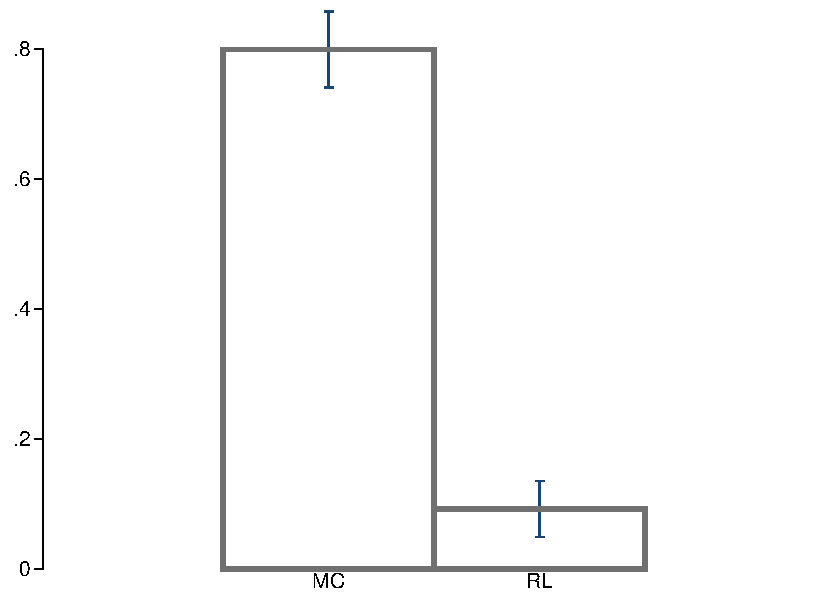
\includegraphics[width=\textwidth]{../figs/relative_score_dt.pdf}
        \caption{Donald Trump}
    \end{subfigure}         
    \caption*{\footnotesize
            Bars indicate the predicted percent of correct responses as reported in \cref{table:study4_results}.  
            MC bar indicates the predicted effect of multiple choice with congenial responses on getting the correct response.
            RL bar indicates the effect of relative scoring with congenial responses on getting the correct response relative to the multiple choice (MC) scheme.
        Capped vertical bars indicate 95\% confidence intervals.
    }
    \label{fig:mturk_relative_score}
\end{figure}

% Commenting out for now
%\begin{table}[t] \centering \small \setlength\tabcolsep{6 pt}
\setlength{\defaultaddspace}{0pt}
  \caption{NEW Results Study 4}
\label{table:study4_results}
%\begin{adjustbox}{max width=\textwidth}
\begin{center}
  \resizebox{\textwidth}{!}{% use resizebox with textwidth
\begin{tabular}{l c c c c c}
  \hline
  & \multicolumn{4}{c}{Individual survey question} \\
  	\cmidrule(l){2-5}
  & Affordable Care Act & Affordable Care Act 2 & Greenhouse Gases & Donald Trump & All \\
  & (1) & (2) & (3) & (4) & (5) \\
\hline
Intercept             & $0.18^{*}$        & $0.21^{*}$        & $0.22^{*}$        & $0.79^{*}$        & $0.29^{*}$        \\
                      & $ [ 0.12;  0.23]$ & $ [ 0.15;  0.27]$ & $ [ 0.16;  0.28]$ & $ [ 0.75;  0.84]$ & $ [ 0.25;  0.32]$ \\
Congenial             & $0.09^{*}$        & $0.08^{*}$        & $0.09^{*}$        & $0.00$            & $0.03$            \\
                      & $ [ 0.02;  0.17]$ & $ [ 0.01;  0.16]$ & $ [ 0.01;  0.17]$ & $ [-0.07;  0.08]$ & $ [-0.02;  0.07]$ \\
Relative Scoring (RS) & $-0.18^{*}$       & $-0.20^{*}$       & $-0.21^{*}$       & $-0.74^{*}$       & $-0.38^{*}$       \\
                      & $ [-0.23; -0.12]$ & $ [-0.26; -0.14]$ & $ [-0.27; -0.14]$ & $ [-0.79; -0.68]$ & $ [-0.41; -0.34]$ \\
Congenial*RL          & $-0.07$           & $-0.07$           & $-0.10^{*}$       & $0.03$            & $0.02$            \\
                      & $ [-0.15;  0.01]$ & $ [-0.15;  0.01]$ & $ [-0.18; -0.02]$ & $ [-0.06;  0.12]$ & $ [-0.03;  0.07]$ \\
  \hline
R$^2$                 & $0.12$            & $0.13$            & $0.15$            & $0.53$            & $0.30$            \\
  Survey item FE        & No                & No                & No                & No                & Yes               \\
Items        & 1                & 1                & 1                & 1                & 4               \\
Respondents             & $902$             & $902$             & $902$             & $902$             & $3608$            \\
Respondent-Items            & $902$             & $902$             & $902$             & $902$             & $902$             \\
\hline
\multicolumn{6}{l}{\scriptsize{$^*$ Null hypothesis value outside the confidence interval.}}
\end{tabular}
}
\end{center}
%\end{adjustbox}
\end{table}


% \cref{fig:mturk_hk} and \cref{tab:mturk_hk} indicate that questionnaire design features might also affect congeniality of responses. Moving from the standard multiple-choice format to the confidence coding comes with a reduction in the congeniality estimate.

% Commenting out for now
\iffalse
% partisan-gaps/scripts/Stata/mturk_hk/mc_likert_coefplot.do
\begin{center}
    \begin{figure}[ht]
        \centering
        \caption{Partisan Gaps in different question designs}
        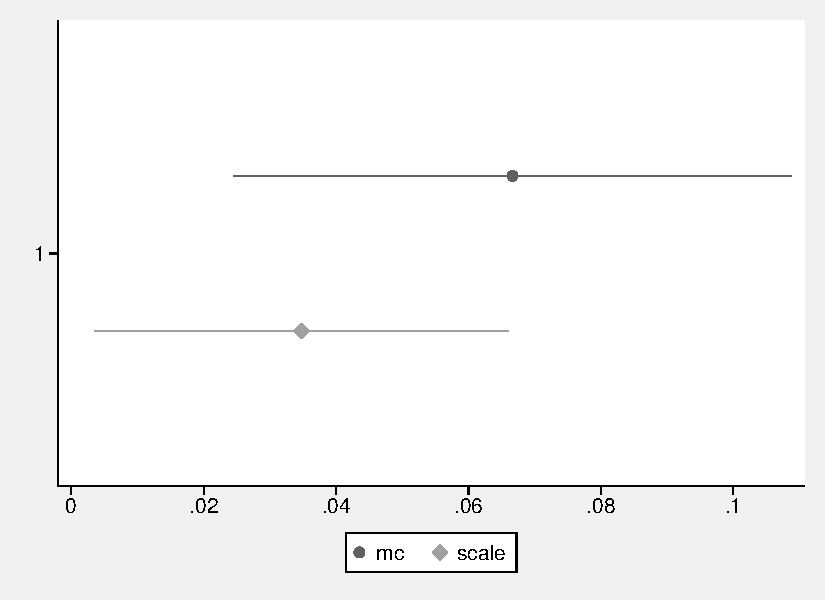
\includegraphics[width=.55\textwidth]{../figs/mturk-hk-MC-LIKERT.pdf}
        \label{fig:mturk_hk}
        \caption*{\scriptsize
            The figure shows the estimated partisan gaps in MTurk 2 for two different survey conditions.
            The multiple-choice condition provides five closed-ended options, including the correct answer and a ``Don't Know''.
            The Likert scale condition only considers the selection of the correct answer with complete confidence of 10 (see \cref{si:mturk2}).
            Estimates correspond to those reported in \cref{tab:mturk_hk}.
            Horizontal bars are 95\% confidence intervals.
        }
    \end{figure}
\end{center}
\fi

% Commenting out for now
%\begin{table}
   \caption{Partisan Gaps in Knowledge in different question designs}
   \label{tab:mturk_hk}
\begin{center}
 \begin{tabular}{l c c}
\hline
   & Condition 4     & Condition 5 \\
   & Multiple Choice & Likert Scale \\
\hline
Congenial      & $0.07^{*}$      & $0.03^{*}$      \\
               & $ [0.02; 0.11]$ & $ [0.00; 0.07]$ \\
(Intercept)    & $0.19^{*}$      & $0.08^{*}$      \\
               & $ [0.15; 0.24]$ & $ [0.05; 0.12]$ \\
\hline
R$^2$          & $0.24$          & $0.25$          \\
Survey item FE & Yes             & Yes             \\
N Clusters     & $480$           & $422$           \\
Num. obs.      & $1920$          & $1688$          \\
\hline
\multicolumn{3}{l}{\scriptsize{$^*$ Null hypothesis value outside the confidence interval.}}
%	\caption*{\scriptsize{All models are linear probability models where the dependent variable indicates whether the response to a survey item is correct. The independent variable indicates whether the partisanship of the respondent is congenial with the content of the questions. The multiple choice model includes four items. Each of these items had four substantive response options with one correct option. All multiple choice questions included ``Don't know''. The Likert Scale items included the same questions as the Multiple Choice items. Here the four substantive questions were presented to the respondents and they were asked to rate on a scale from 0-10 how true each statement is. Answers were coded as correct for individuals that indicated 10 for the correct statement. Results are robust to a specification that codes greater than 7 as correct.  All models include survey item fixed effects. Standard errors are clustered at the respondent level.}}
  \end{tabular}
\end{center}
\end{table}


% partisan-gaps/scripts/Stata/mturk_hk/reg-table.do
\begin{table}[t] \centering \small \setlength\tabcolsep{6 pt} \setlength{\defaultaddspace}{0pt}
    \def\sym#1{\ifmmode^{#1}\else\(^{#1}\)\fi}
    \caption{Confidence Scoring and Knowledge Gaps: MTurk 2} 
    \label{table:study4_results}
    \begin{adjustbox}{max width=\textwidth}
        \begin{tabular}{@{\hspace{0\tabcolsep}}l*{6}{D{.}{.}{-1}}@{\hspace{0\tabcolsep}}}
            \toprule
            % https://tex.stackexchange.com/questions/567985/problems-with-inputtable-tex-hline-after-2020-fall-latex-release
            &\multicolumn{4}{c}{Individual survey question}\\
            \cmidrule(l){2-5}
            &\multicolumn{1}{c}{Affordable Care Act}&\multicolumn{1}{c}{Affordable Care Act 2}&\multicolumn{1}{c}{Greenhouse gases}&\multicolumn{1}{c}{Donald Trump}&\multicolumn{1}{c}{All}\\
            \input ../tabs/mturk-hk-reg-table-fragment.tex
            \bottomrule
        \end{tabular}
    \end{adjustbox}
    \caption*{\scriptsize Dependent variables indicate whether the respondent answered the question(s) correctly. 
        See \cref{si:mturk2} for the exact wording of the four questions.
        Columns (1)--(4) estimates by the individual survey questions.
        Column (5) includes all questions and adds the survey question fixed effects.
        All models are linear probability models.
        In the relative scoring scheme, a response is correct only if the correct answer is selected with full confidence of 10 (see \nameref{sec:data3} in the \nameref{sec:confidence_coding} section).
        The baseline is the multiple choice designs. \cref{tab:tab6_robustness} implements a robustness check setting the relative scoring threshold to 8. Standard errors are clustered at the respondent level. Significance levels: + 0.1 * 0.05 ** 0.01 *** 0.001.}
\end{table}

\clearpage

\section*{Validity and Reliability of Question Designs}
\label{sec:validation}

Till now, we have shown that survey and item design choices that encourage guessing have larger partisan gaps than ones that discourage guessing and where the scoring scheme codes only confident answers as evidence of knowledge. But which item and survey design choices lead to 'better' measures? The presumption is that better political knowledge measures are also better instruments for measuring partisan gaps. 

To answer which design choices lead to better measures, we use data from the first MTurk survey to assess the reliability and criterion validity of different designs. Specifically, we use average inter-item correlation and Cronbach's $\alpha$ to measure the reliability of the scale. To measure criterion validity, we use the correlation of the scale with three criteria thought to correlate heavily with political knowledge: education, political interest, and political participation (see SI \ref{si:mturk1_criteria} for the question text). Our expectation is that items that discourage guessing will have higher reliability and greater criterion validity. 

\cref{tab:criterion-var-corr} reports results for each of the four conditions (see \cref{tab:conditions}) and the confidence coding condition (CCD) that scores a response as correct when the respondent is completely confident about the correct answer. CCD has better reliability than other versions. However, the picture is more mixed for the other conditions with FSR and IDA having greater reliability than CUD and IMC. One of the reasons for this mixed picture may be that partisan guessing increases reliability without increasing validity because it introduces correlated error. A more diagnostic test for the quality of the instrument hence is criterion validity. As Panel A of \cref{tab:criterion-var-corr} shows, the average correlation between IMC and CCD and criterion variables is markedly higher (~ .34) than IDA (.11), CUD (.20), and FSR (.26).\footnote{We did one more test to get at the validity. We hypothesized that partisan guessing would lead to a greater negative correlation between congenial and uncongenial items on items that encouraged guessing. And indeed the item-rest correlations between uncongenial and congenial items are the smallest for CCD.)}

\begin{table}[ht] \centering \normalsize \setlength\tabcolsep{6 pt} \setlength{\defaultaddspace}{0pt}
    \def\sym#1{\ifmmode^{#1}\else\(^{#1}\)\fi}
    \caption{Validity and Reliability}
    \label{tab:criterion-var-corr}
    \begin{adjustbox}{max width=\textwidth}
        \begin{tabular}{@{\hspace{0\tabcolsep}}l*{6}{D{.}{.}{-1}}@{\hspace{0\tabcolsep}}}
            \toprule    
                &\multicolumn{5}{c}{\textbf{Conditions}}\\
                &\multicolumn{2}{c}{No DK}&\multicolumn{3}{c}{With DK}\\
                \cmidrule(lr){2-3}\cmidrule(l){4-6}
                &\multicolumn{1}{c}{IDA}&\multicolumn{1}{c}{CUD}&\multicolumn{1}{c}{FSR}&\multicolumn{1}{c}{IMC}&\multicolumn{1}{c}{CCD}\\                
                &\multicolumn{1}{c}{(1)}&\multicolumn{1}{c}{(2)}         &\multicolumn{1}{c}{(3)}&\multicolumn{1}{c}{(4)}         &\multicolumn{1}{c}{(5)}\\
                \midrule
                &\multicolumn{5}{c}{\textbf{Panel A.} Criterion correlational validity}\\
                \cmidrule(l){2-6}
                % Criterion by condition --- correlations
                Political interest      &.115&.278&.271&.412&.379 \tabularnewline
                Political participation &.138&.168&.276&.298&.356 \tabularnewline
                Education               &.077&.167&.23&.18&.302 \tabularnewline
                &\multicolumn{5}{c}{\textbf{Panel B.} Inter-item correlation}\\
                \cmidrule(l){2-6}
                Average inter-item correlation&.237&.163&.248&.172&.325\\
                \cmidrule(l){2-6}
                &\multicolumn{5}{c}{\textbf{Panel C.} Scale reliability}\\
                \cmidrule(l){2-6}
                Cronbach's alpha&.737&.637&.748&.652&.812\\
            \bottomrule
        \end{tabular}
    \end{adjustbox}
    \caption*{\footnotesize 
            Panel A reports the correlation coefficient between each condition and the three criterion variables. 
            Political interest and political participation (voting) are coded on an 11-point scale. Education is coded from 1--5 by education qualification. 
            Panel B reports the inter-item correlation for the nine items (see \cref{fig:partisangaps-mturk}).
            Panel C reports the Cronbach's alpha coefficient of scale reliability for the nine items.
            See \cref{tab:conditions} for a brief description of the first four conditions and \nameref{sec:confidence_coding} for the confidence coding design.
        }
\end{table}

The results obtained above are consistent with those obtained by \citet{graham2021measuring} who finds that the test-retest reliability of confident correct answers is much higher. In all, the data suggest that the substantially smaller partisan gap that we see in CCD is also the best estimate of the partisan gap.

\section*{Discussion and Conclusion}\label{sec:discussion}

Since at least the publication of \cite{bartels_2002}, the conventional wisdom has been that partisan gaps in beliefs about politically consequential facts are both wide and widespread. The conventional wisdom in academia has also become the received wisdom for the mass public---nearly 80\% of Americans believe that Democrats and Republicans disagree on facts \citep{pew2018disagree}.

In line with some other research on this topic \citep[][though see \citeauthor{berinsky_2017} \citeyear{berinsky_2017} and \citeauthor{peterson_iyengar_forth} \citeyear{peterson_iyengar_forth}]{bullocketal_2015, prior2015you, schaffner_luks}, our results suggest that a big chunk of the partisan gap is not founded in differences in beliefs. We find that common features of commercial polls like not asking don't know, inserting a partisan cue, and treating unconfident answers as knowledge inflate the partisan gaps.

The fact that partisan gaps are smaller may seem at odds with some political behavior research. For instance, the theory of selective exposure posits vast imbalances in the consumption of partisan news. However, recent studies show that most people consume scant political news \citep{Prior2007,flaxmanetal_2016}, and the news that they do consume is relatively balanced \citep{flaxmanetal_2016,garzetal_2018,gentzkowshapiro_2011,guess_2020}. Other evidence points to the fact that Democrats and Republicans update similarly in light of events \citep{gerber_annual_review,kernell_2019, coppock2021persuasion}.

In the end, the results paint a mixed picture of democratic competence. Smaller partisan gaps are partly a consequence of the fact that the average respondent doesn't know the facts. It is mostly partisan guessing masquerading as partisan gaps. The upside is that partisan gaps are small, and the downside is that people know even less than we thought.

\clearpage
\bibliographystyle{apsr}
\bibliography{pgap}

\clearpage


\appendix
\renewcommand{\thesection}{SI \arabic{section}}
\setcounter{table}{0}\renewcommand\thetable{\thesection.\arabic{table}}
\setcounter{figure}{0}\renewcommand\thefigure{\thesection.\arabic{figure}}
\counterwithin{figure}{section}


\begin{center}
\Large \textbf{Supporting Information}
\end{center}
\singlespacing
\vspace{-.4in}

\section{Balance Tests}\label{si:baltests}

\begin{center}
	\begin{figure}[H]
		\centering
		\caption{MTurk 1---IDA and CUD}
		\includegraphics[width=\textwidth]{../figs/study1-baltest-RW-ips.pdf}
		\label{fig:baltest-RW-ips}
		\caption*{\footnotesize 
			Figure shows the balance tests of respondent characteristics for the Amazon Mechanical Turk Study 1 sample.
			The tests compare respondents assigned to the IDA condition vs. respondents assigned to the CUD condition.
			See \cref{tab:conditions} in \nameref{sec:inflationary_measures}.
			Rows are self-reported characteristics.
		      The second column reports the estimates from regressing the characteristics on the CUD dummy, with IDA as the baseline.
		      The third column reports the p-values.
			Horizontal bars are 95\% confidence intervals constructed from robust standard errors.
		}
	\end{figure}
\end{center}

% MTurk 1 balance test: IDA vs FSR (IPS vs FSR)
\begin{center}
	\begin{figure}
		\centering
		\caption{MTurk 1---IDA and FSR}
		\includegraphics[width=\textwidth]{../figs/study1-baltest-FSR-ips.pdf}
		\label{fig:baltest-FSR-ips}
		\caption*{\footnotesize 
			Figure shows the balance tests of respondent characteristics for the Amazon Mechanical Turk Study 1 sample.
			The tests compare respondents assigned to the IDA condition vs. respondents assigned to the FSR condition.
			See \cref{tab:conditions} in \nameref{sec:inflationary_measures}.
			Rows are self-reported characteristics.
			The second column reports the estimates from regressing the characteristics on the FSR dummy, with IDA as the baseline.
			The third column reports the p-values.
			Horizontal bars are 95\% confidence intervals constructed from robust standard errors.
		}
	\end{figure}
\end{center}

\begin{center}
	\begin{figure}
		\centering
		\caption{MTurk 1---IDA and IMC}
		\includegraphics[width=\textwidth]{../figs/study1-baltest-14k-ips.pdf}
		\label{fig:baltest-14k-ips}
		\caption*{\footnotesize 
			Figure shows the balance tests of respondent characteristics for the Amazon Mechanical Turk Study 1 sample.
			The tests compare respondents assigned to the IDA condition vs. respondents assigned to the IMC condition.
			See \cref{tab:conditions} in \nameref{sec:inflationary_measures}.
			Rows are self-reported characteristics.
			The second column reports the estimates from regressing the characteristics on the IMC dummy, with IDA as the baseline.
			The third column reports the p-values.
			Horizontal bars are 95\% confidence intervals constructed from robust standard errors.
		}
	\end{figure}
\end{center}

\begin{center}
	\begin{figure}
		\centering
		\caption{MTurk 1---IDA and CCD}
		\includegraphics[width=\textwidth]{../figs/study1-baltest-24k-ips.pdf}
		\label{fig:baltest-24k-ips}
		\caption*{\footnotesize 
			Figure shows the balance tests of respondent characteristics for the Amazon Mechanical Turk Study 1 sample.
			The tests compare respondents assigned to the IDA condition vs. respondents assigned to the CCD condition.
			See \cref{tab:conditions} in \nameref{sec:inflationary_measures}.
			Rows are self-reported characteristics.
			The second column reports the estimates from regressing the characteristics on the CCD dummy, with IDA as the baseline.
			The third column reports the p-values.
			Horizontal bars are 95\% confidence intervals constructed from robust standard errors.
		}
	\end{figure}
\end{center}

\section{Partisan Knowledge Gaps with Partisan Cues: YouGov}

\begin{figure}[ht]
	\caption{Partisan Knowledge Gaps with Partisan Cues: YouGov}
	\centering
	\begin{subfigure}{.495\textwidth}\centering
		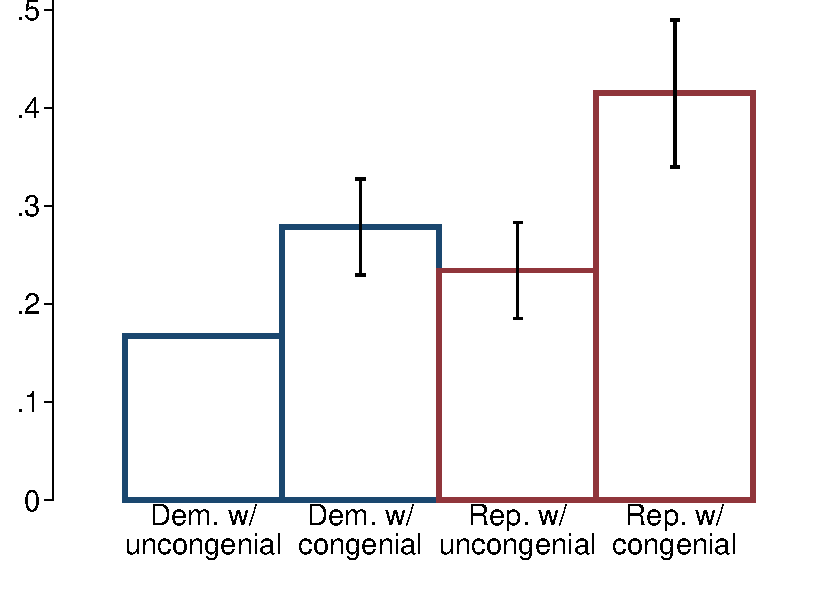
\includegraphics[width=\textwidth]{../figs/yougov-unemp-congenialcue-partisan.pdf}
		\caption{Unemployment}
	\end{subfigure}
	\hfil
	\begin{subfigure}{.495\textwidth}\centering
		\includegraphics[width=\textwidth]{../figs/yougov-deficit-congenialcue-partisan.pdf}
		\caption{Budget deficit}
	\end{subfigure}
	\caption*{\footnotesize Figure shows the effect of congenial cues for the YouGov survey by partisanship. Bars indicate the predicted percent of responses saying that unemployment has gone up (correct response) as retrieved from the estimates in \cref{tab:partisangaps-yougov} (columns (2) and (5)).  The estimates are obtained by estimating:\\

	$\qquad\text{correct response}_{i} = \alpha + \beta (congenial \; cue)_i + \gamma (Rep)_i + \delta (congenial\; cue \times Rep)_i + \varepsilon_{i}$.\\

	Capped vertical bars indicate 95\% confidence intervals.
	}
	\label{fig:yougov-reg-by-partisanship}
\end{figure}

\clearpage
\section{Confidence Scoring for Mturk 1}\label{si:mturk1-ccd}

\begin{table}[th] \centering \small \setlength\tabcolsep{0 pt} \setlength{\defaultaddspace}{0pt}
	\def\sym#1{\ifmmode^{#1}\else\(^{#1}\)\fi}
	\caption{Confidence Scoring vs. Other Survey Conditions (MTurk 1)}
	\label{tab:confidence-scoring-study1}
	\begin{adjustbox}{max width=\textwidth}
		\begin{tabular}{l*{10}{D{.}{.}{-1}}}
			\toprule
			&\multicolumn{1}{c}{Obama}
			&\multicolumn{1}{c}{Obama}
			&\multicolumn{1}{c}{ACA}
			&\multicolumn{1}{c}{ACA death}
			&\multicolumn{1}{c}{GW causes}
			&\multicolumn{1}{c}{GW scientists}
			&\multicolumn{1}{c}{Voter}
			&\multicolumn{1}{c}{MMR}
			&\multicolumn{1}{c}{Budget}
			&\multicolumn{1}{c}{}
			\\
			&\multicolumn{1}{c}{birthplace}
			&\multicolumn{1}{c}{religion}
			&\multicolumn{1}{c}{illegal}
			&\multicolumn{1}{c}{panels}
			&\multicolumn{1}{c}{GW causes}
			&\multicolumn{1}{c}{agree}
			&\multicolumn{1}{c}{fraud}
			&\multicolumn{1}{c}{vaccine}
			&\multicolumn{1}{c}{deficit}
			&\multicolumn{1}{c}{All}
			\\			
			\cmidrule(l){2-10}
			\input ../tabs/confidence-scoring-study1-fragment.tex
			\bottomrule
		\end{tabular}
	\end{adjustbox}
	\caption*{\scriptsize 
		All models are linear probability models where the dependent variable indicates whether the response to a survey item is correct.
		Under the Confidence Scoring condition, we only consider responses as correct when they are chosen with complete confidence (10 on a 0--10 scale).
		The baseline conditions are the IDA, CUD, FSR, and IMC conditions pooled together (see \cref{tab:conditions} for the descriptions).
		Columns (1)--(9) are for each of the survey questions.
		The model in column (10) pools all nine survey questions.
		See \cref{table:study4_results} for a similar result using MTurk 2.
		See \crefrange{tab:confidence-scoring-study1-ccd-ida-ips}{tab:confidence-scoring-study1-ccd-14k-imc} for the results comparing the Confidence Scoring condition to each of the four other individual survey conditions.
		See \cref{fig:confidence-scoring-study1} for the visualization of how Confidence Scoring mediates the effect that congenial responses have.
		Standard errors are clustered at the respondent level. 
		Significance levels: + 0.1 * 0.05 ** 0.01 *** 0.001.}
\end{table}

\begin{table}[t] \centering \small \setlength\tabcolsep{0 pt} \setlength{\defaultaddspace}{0pt}
	\def\sym#1{\ifmmode^{#1}\else\(^{#1}\)\fi}
	\caption{Confidence Scoring vs. IDA (MTurk 1)}
	\label{tab:confidence-scoring-study1-ccd-ida-ips}
	\begin{adjustbox}{max width=\textwidth}
		\begin{tabular}{l*{10}{D{.}{.}{-1}}}
			\toprule
			&\multicolumn{1}{c}{Obama}
			&\multicolumn{1}{c}{Obama}
			&\multicolumn{1}{c}{ACA}
			&\multicolumn{1}{c}{ACA death}
			&\multicolumn{1}{c}{GW causes}
			&\multicolumn{1}{c}{GW scientists}
			&\multicolumn{1}{c}{Voter}
			&\multicolumn{1}{c}{MMR}
			&\multicolumn{1}{c}{Budget}
			&\multicolumn{1}{c}{}
			\\
			&\multicolumn{1}{c}{birthplace}
			&\multicolumn{1}{c}{religion}
			&\multicolumn{1}{c}{illegal}
			&\multicolumn{1}{c}{panels}
			&\multicolumn{1}{c}{GW causes}
			&\multicolumn{1}{c}{agree}
			&\multicolumn{1}{c}{fraud}
			&\multicolumn{1}{c}{vaccine}
			&\multicolumn{1}{c}{deficit}
			&\multicolumn{1}{c}{All}
			\\			
			\cmidrule(l){2-10}
			\input ../tabs/confidence-scoring-study1-ccd-ida-ips-fragment.tex
			\bottomrule
		\end{tabular}
	\end{adjustbox}
	\caption*{\scriptsize 
		All models are linear probability models where the dependent variable indicates whether the response to a survey item is correct.
		Under the Confidence Scoring condition, we only consider responses as correct when they are chosen with complete confidence (10 on a 0--10 scale).
		The baseline condition is the IDA condition (see \cref{tab:conditions} for the descriptions).
		Columns (1)--(9) are for each of the survey questions.
		The model in column (10) pools all nine survey questions.
		See \cref{table:study4_results} for a similar result using MTurk 2.
		See \cref{tab:confidence-scoring-study1} for the results comparing the Confidence Scoring condition with all the four other conditions (IDA, CUD, FSR, IMC) pooled together.
		See \cref{fig:confidence-scoring-study1-ccd-ida-ips} for the visualization of how Confidence scoring mediates the effect that congenial responses have.
		See \cref{fig:confidence-scoring-study1-ccd-ida-ips} for the visualization of how Confidence scoring mediates the effect that congenial responses have.
		Standard errors are clustered at the respondent level. 
		Significance levels: + 0.1 * 0.05 ** 0.01 *** 0.001.}
\end{table}

\begin{table}[t] \centering \small \setlength\tabcolsep{0 pt} \setlength{\defaultaddspace}{0pt}
	\def\sym#1{\ifmmode^{#1}\else\(^{#1}\)\fi}
	\caption{Confidence Scoring vs. CUD (MTurk 1)}
	\label{tab:confidence-scoring-study1-ccd-rw-cud}
	\begin{adjustbox}{max width=\textwidth}
		\begin{tabular}{l*{10}{D{.}{.}{-1}}}
			\toprule
			&\multicolumn{1}{c}{Obama}
			&\multicolumn{1}{c}{Obama}
			&\multicolumn{1}{c}{ACA}
			&\multicolumn{1}{c}{ACA death}
			&\multicolumn{1}{c}{GW causes}
			&\multicolumn{1}{c}{GW scientists}
			&\multicolumn{1}{c}{Voter}
			&\multicolumn{1}{c}{MMR}
			&\multicolumn{1}{c}{Budget}
			&\multicolumn{1}{c}{}
			\\
			&\multicolumn{1}{c}{birthplace}
			&\multicolumn{1}{c}{religion}
			&\multicolumn{1}{c}{illegal}
			&\multicolumn{1}{c}{panels}
			&\multicolumn{1}{c}{GW causes}
			&\multicolumn{1}{c}{agree}
			&\multicolumn{1}{c}{fraud}
			&\multicolumn{1}{c}{vaccine}
			&\multicolumn{1}{c}{deficit}
			&\multicolumn{1}{c}{All}
			\\			
			\cmidrule(l){2-10}
			\input ../tabs/confidence-scoring-study1-ccd-cud-rw-fragment.tex
			\bottomrule
		\end{tabular}
	\end{adjustbox}
	\caption*{\scriptsize 
		All models are linear probability models where the dependent variable indicates whether the response to a survey item is correct.
		Under the Confidence Scoring condition, we only consider responses as correct when they are chosen with complete confidence (10 on a 0--10 scale).
		The baseline condition is the CUD condition (see \cref{tab:conditions} for the descriptions).
		Columns (1)--(9) are for each of the survey questions.
		The model in column (10) pools all nine survey questions.
		See \cref{table:study4_results} for a similar result using MTurk 2.
		See \cref{tab:confidence-scoring-study1} for the results comparing the Confidence scoring condition with all the four other conditions (IDA, CUD, FSR, IMC) pooled together.
		See \cref{fig:confidence-scoring-study1-ccd-rw-cud} for the visualization of how Confidence scoring mediates the effect that congenial responses have.
		Standard errors are clustered at the respondent level. 
		Significance levels: + 0.1 * 0.05 ** 0.01 *** 0.001.}
\end{table}


\begin{table}[t] \centering \small \setlength\tabcolsep{0 pt} \setlength{\defaultaddspace}{0pt}
	\def\sym#1{\ifmmode^{#1}\else\(^{#1}\)\fi}
	\caption{Confidence Scoring vs. FSR (MTurk 1)}
	\label{tab:confidence-scoring-study1-ccd-fsr-fsr}
	\begin{adjustbox}{max width=\textwidth}
		\begin{tabular}{l*{10}{D{.}{.}{-1}}}
			\toprule
			&\multicolumn{1}{c}{Obama}
			&\multicolumn{1}{c}{Obama}
			&\multicolumn{1}{c}{ACA}
			&\multicolumn{1}{c}{ACA death}
			&\multicolumn{1}{c}{GW causes}
			&\multicolumn{1}{c}{GW scientists}
			&\multicolumn{1}{c}{Voter}
			&\multicolumn{1}{c}{MMR}
			&\multicolumn{1}{c}{Budget}
			&\multicolumn{1}{c}{}
			\\
			&\multicolumn{1}{c}{birthplace}
			&\multicolumn{1}{c}{religion}
			&\multicolumn{1}{c}{illegal}
			&\multicolumn{1}{c}{panels}
			&\multicolumn{1}{c}{GW causes}
			&\multicolumn{1}{c}{agree}
			&\multicolumn{1}{c}{fraud}
			&\multicolumn{1}{c}{vaccine}
			&\multicolumn{1}{c}{deficit}
			&\multicolumn{1}{c}{All}
			\\			
			\cmidrule(l){2-10}
			\input ../tabs/confidence-scoring-study1-ccd-fsr-fsr-fragment.tex
			\bottomrule
		\end{tabular}
	\end{adjustbox}
	\caption*{\scriptsize 
		All models are linear probability models where the dependent variable indicates whether the response to a survey item is correct.
		Under the Confidence Scoring condition, we only consider responses as correct when they are chosen with complete confidence (10 on a 0--10 scale).
		The baseline condition is the FSR condition (see \cref{tab:conditions} for the descriptions).
		Columns (1)--(9) are for each of the survey questions.
		The model in column (10) pools all nine survey questions.
		See \cref{table:study4_results} for a similar result using MTurk 2.
		See \cref{tab:confidence-scoring-study1} for the results comparing the Confidence Scoring condition with all the four other conditions (IDA, CUD, FSR, IMC) pooled together.
		See \cref{fig:confidence-scoring-study1-ccd-fsr-fsr} for the visualization of how Confidence Scoring mediates the effect that congenial responses have.
		Standard errors are clustered at the respondent level. 
		Significance levels: + 0.1 * 0.05 ** 0.01 *** 0.001.}
\end{table}


\begin{table}[t] \centering \small \setlength\tabcolsep{0 pt} \setlength{\defaultaddspace}{0pt}
	\def\sym#1{\ifmmode^{#1}\else\(^{#1}\)\fi}
	\caption{Confidence Scoring vs. IMC (MTurk 1)}
	\label{tab:confidence-scoring-study1-ccd-14k-imc}
	\begin{adjustbox}{max width=\textwidth}
		\begin{tabular}{l*{10}{D{.}{.}{-1}}}
			\toprule
			&\multicolumn{1}{c}{Obama}
			&\multicolumn{1}{c}{Obama}
			&\multicolumn{1}{c}{ACA}
			&\multicolumn{1}{c}{ACA death}
			&\multicolumn{1}{c}{GW causes}
			&\multicolumn{1}{c}{GW scientists}
			&\multicolumn{1}{c}{Voter}
			&\multicolumn{1}{c}{MMR}
			&\multicolumn{1}{c}{Budget}
			&\multicolumn{1}{c}{}
			\\
			&\multicolumn{1}{c}{birthplace}
			&\multicolumn{1}{c}{religion}
			&\multicolumn{1}{c}{illegal}
			&\multicolumn{1}{c}{panels}
			&\multicolumn{1}{c}{GW causes}
			&\multicolumn{1}{c}{agree}
			&\multicolumn{1}{c}{fraud}
			&\multicolumn{1}{c}{vaccine}
			&\multicolumn{1}{c}{deficit}
			&\multicolumn{1}{c}{All}
			\\			
			\cmidrule(l){2-10}
			\input ../tabs/confidence-scoring-study1-ccd-imc-14k-fragment.tex
			\bottomrule
		\end{tabular}
	\end{adjustbox}
	\caption*{\scriptsize 
		All models are linear probability models where the dependent variable indicates whether the response to a survey item is correct.
		Under the Confidence Scoring condition, we only consider responses as correct when they are chosen with complete confidence (10 on a 0--10 scale).
		The baseline condition is the IMC condition (see \cref{tab:conditions} for the descriptions).
		Columns (1)--(9) are for each of the survey questions.
		The model in column (10) pools all nine survey questions.
		See \cref{table:study4_results} for a similar result using MTurk 2.
		See \cref{tab:confidence-scoring-study1} for the results comparing the Confidence Scoring condition with all the four other conditions (IDA, CUD, FSR, IMC) pooled together.
		See \cref{fig:confidence-scoring-study1-ccd-imc-14k} for the visualization of how Confidence Scoring mediates the effect that congenial responses have.
		Standard errors are clustered at the respondent level. 
		Significance levels: + 0.1 * 0.05 ** 0.01 *** 0.001.}
\end{table}


\begin{figure}[t]
	\caption{Confidence Scoring vs. Other Survey Conditions (MTurk 1)}	
	\centering
	% First row a
	\begin{subfigure}{.325\textwidth}\centering
		\includegraphics[width=\textwidth]{../figs/confidence_score_birth_study1.pdf}
		\caption{Obama birthplace}
	\end{subfigure}
	\hfill
	% First row b
	\begin{subfigure}{.325\textwidth}\centering
		\includegraphics[width=\textwidth]{../figs/confidence_score_religion_study1.pdf}
		\caption{Obama religion}
	\end{subfigure}	
	\hfill
	% First row c
	\begin{subfigure}{.325\textwidth}\centering
		\includegraphics[width=\textwidth]{../figs/confidence_score_illegal_study1.pdf}
		\caption{ACA illegal}
	\end{subfigure}	
	% Second row a
	\begin{subfigure}{.325\textwidth}\centering
		\includegraphics[width=\textwidth]{../figs/confidence_score_death_study1.pdf}
		\caption{ACA death panels}
	\end{subfigure}
	\hfill
	% Second row b
	\begin{subfigure}{.325\textwidth}\centering
		\includegraphics[width=\textwidth]{../figs/confidence_score_increase_study1.pdf}
		\caption{GW causes}
	\end{subfigure}	
	\hfill
	% Second row c
	\begin{subfigure}{.325\textwidth}\centering
		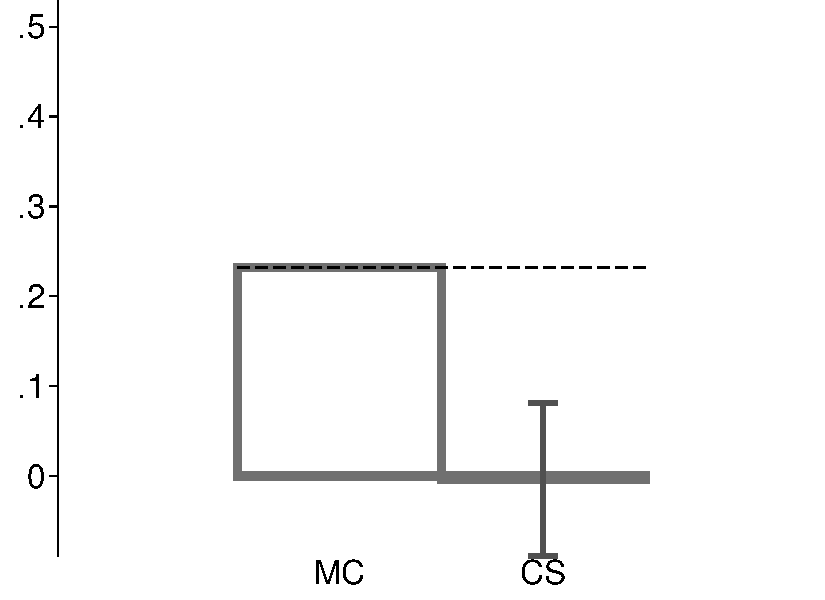
\includegraphics[width=\textwidth]{../figs/confidence_score_science_study1.pdf}
		\caption{GW scientists agree}
	\end{subfigure}	
	% Third row a
	\begin{subfigure}{.325\textwidth}\centering
		\includegraphics[width=\textwidth]{../figs/confidence_score_fraud_study1.pdf}
		\caption{Voter fraud}
	\end{subfigure}
	\hfill
	% Third row b
	\begin{subfigure}{.325\textwidth}\centering
		\includegraphics[width=\textwidth]{../figs/confidence_score_mmr_study1.pdf}
		\caption{MMR vaccine}
	\end{subfigure}	
	\hfill
	% Third row c
	\begin{subfigure}{.325\textwidth}\centering
		\includegraphics[width=\textwidth]{../figs/confidence_score_deficit_study1.pdf}
		\caption{Budget deficit}
	\end{subfigure}	
	\caption*{\footnotesize 
		Bars indicate the predicted percent of correct responses when the correct response is congenial to the party, depending on whether the survey condition is based on Confidence Scoring (CS) or from Multiple Choice conditions (IDA, CUD, FSR, IMC; see \cref{tab:conditions} for the descriptions).
		Reconstructed from the estimates from \cref{tab:confidence-scoring-study1}.
		Capped vertical bars indicate 95\% confidence intervals.
	}
	\label{fig:confidence-scoring-study1}
\end{figure}


\begin{figure}[t]
	\caption{Confidence Scoring vs. IDA (MTurk 1)}	
	\centering
	% First row a
	\begin{subfigure}{.325\textwidth}\centering
		\includegraphics[width=\textwidth]{../figs/confidence_score_ccd_ida_ips_birth_study1.pdf}
		\caption{Obama birthplace}
	\end{subfigure}
	\hfill
	% First row b
	\begin{subfigure}{.325\textwidth}\centering
		\includegraphics[width=\textwidth]{../figs/confidence_score_ccd_ida_ips_religion_study1.pdf}
		\caption{Obama religion}
	\end{subfigure}	
	\hfill
	% First row c
	\begin{subfigure}{.325\textwidth}\centering
		\includegraphics[width=\textwidth]{../figs/confidence_score_ccd_ida_ips_illegal_study1.pdf}
		\caption{ACA illegal}
	\end{subfigure}	
	% Second row a
	\begin{subfigure}{.325\textwidth}\centering
		\includegraphics[width=\textwidth]{../figs/confidence_score_ccd_ida_ips_death_study1.pdf}
		\caption{ACA death panels}
	\end{subfigure}
	\hfill
	% Second row b
	\begin{subfigure}{.325\textwidth}\centering
		\includegraphics[width=\textwidth]{../figs/confidence_score_ccd_ida_ips_increase_study1.pdf}
		\caption{GW causes}
	\end{subfigure}	
	\hfill
	% Second row c
	\begin{subfigure}{.325\textwidth}\centering
		\includegraphics[width=\textwidth]{../figs/confidence_score_ccd_ida_ips_science_study1.pdf}
		\caption{GW scientists agree}
	\end{subfigure}	
	% Third row a
	\begin{subfigure}{.325\textwidth}\centering
		\includegraphics[width=\textwidth]{../figs/confidence_score_ccd_ida_ips_fraud_study1.pdf}
		\caption{Voter fraud}
	\end{subfigure}
	\hfill
	% Third row b
	\begin{subfigure}{.325\textwidth}\centering
		\includegraphics[width=\textwidth]{../figs/confidence_score_ccd_ida_ips_mmr_study1.pdf}
		\caption{MMR vaccine}
	\end{subfigure}	
	\hfill
	% Third row c
	\begin{subfigure}{.325\textwidth}\centering
		\includegraphics[width=\textwidth]{../figs/confidence_score_ccd_ida_ips_deficit_study1.pdf}
		\caption{Budget deficit}
	\end{subfigure}	
	\caption*{\footnotesize 
		Bars indicate the predicted percent of correct responses when the correct response is congenial to the party, depending on whether the survey condition is based on Confidence Scoring (CS) or from multiple choice IDA condition (see \cref{tab:conditions} for the descriptions).
		Reconstructed from the estimates from \cref{tab:confidence-scoring-study1-ccd-ida-ips}.
		Capped vertical bars indicate 95\% confidence intervals.
	}
	\label{fig:confidence-scoring-study1-ccd-ida-ips}
\end{figure}


\begin{figure}[t]
	\caption{Confidence Scoring vs. CUD (MTurk 1)}	
	\centering
	% First row a
	\begin{subfigure}{.325\textwidth}\centering
		\includegraphics[width=\textwidth]{../figs/confidence_score_ccd_cud_rw_birth_study1.pdf}
		\caption{Obama birthplace}
	\end{subfigure}
	\hfill
	% First row b
	\begin{subfigure}{.325\textwidth}\centering
		\includegraphics[width=\textwidth]{../figs/confidence_score_ccd_cud_rw_religion_study1.pdf}
		\caption{Obama religion}
	\end{subfigure}	
	\hfill
	% First row c
	\begin{subfigure}{.325\textwidth}\centering
		\includegraphics[width=\textwidth]{../figs/confidence_score_ccd_cud_rw_illegal_study1.pdf}
		\caption{ACA illegal}
	\end{subfigure}	
	% Second row a
	\begin{subfigure}{.325\textwidth}\centering
		\includegraphics[width=\textwidth]{../figs/confidence_score_ccd_cud_rw_death_study1.pdf}
		\caption{ACA death panels}
	\end{subfigure}
	\hfill
	% Second row b
	\begin{subfigure}{.325\textwidth}\centering
		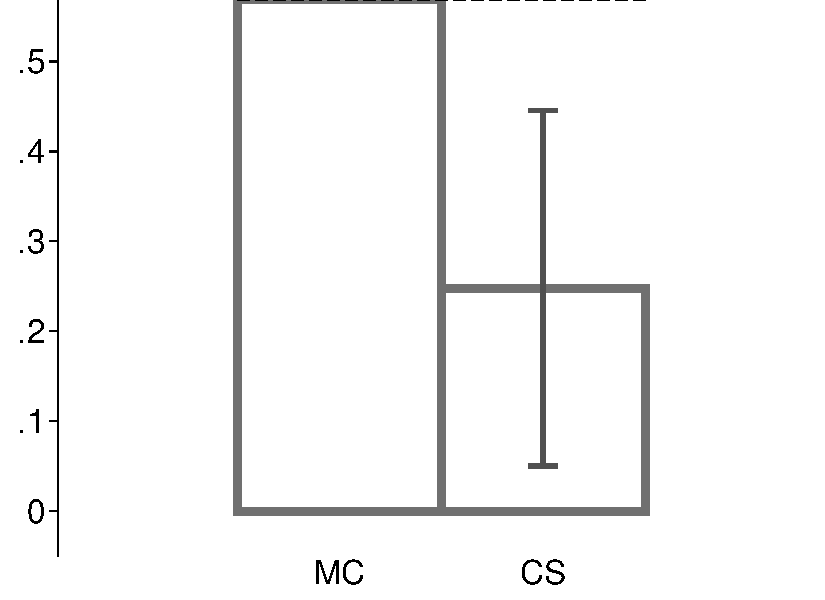
\includegraphics[width=\textwidth]{../figs/confidence_score_ccd_cud_rw_increase_study1.pdf}
		\caption{GW causes}
	\end{subfigure}	
	\hfill
	% Second row c
	\begin{subfigure}{.325\textwidth}\centering
		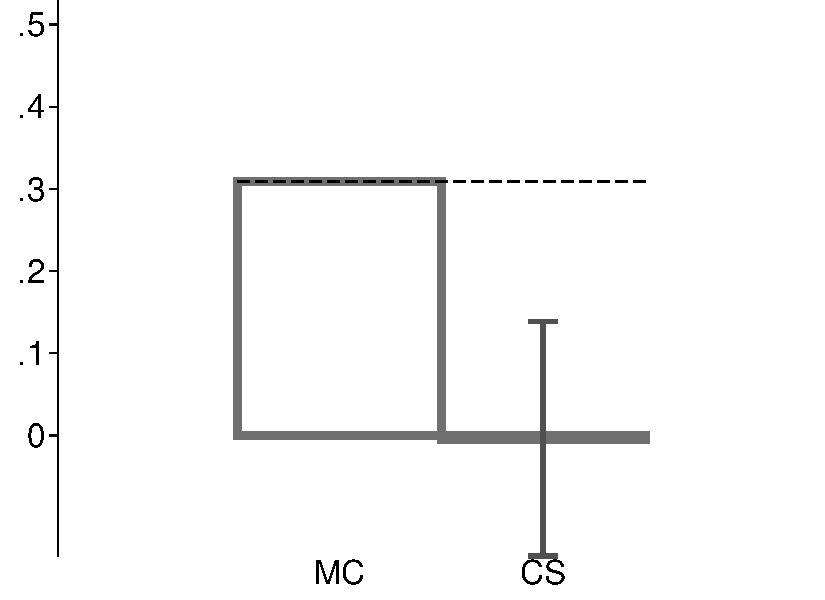
\includegraphics[width=\textwidth]{../figs/confidence_score_ccd_cud_rw_science_study1.pdf}
		\caption{GW scientists agree}
	\end{subfigure}	
	% Third row a
	\begin{subfigure}{.325\textwidth}\centering
		\includegraphics[width=\textwidth]{../figs/confidence_score_ccd_cud_rw_fraud_study1.pdf}
		\caption{Voter fraud}
	\end{subfigure}
	\hfill
	% Third row b
	\begin{subfigure}{.325\textwidth}\centering
		\includegraphics[width=\textwidth]{../figs/confidence_score_ccd_cud_rw_mmr_study1.pdf}
		\caption{MMR vaccine}
	\end{subfigure}	
	\hfill
	% Third row c
	\begin{subfigure}{.325\textwidth}\centering
		\includegraphics[width=\textwidth]{../figs/confidence_score_ccd_cud_rw_deficit_study1.pdf}
		\caption{Budget deficit}
	\end{subfigure}	
	\caption*{\footnotesize 
		Bars indicate the predicted percent of correct responses when the correct response is congenial to the party, depending on whether the survey condition is based on Confidence Scoring (CS) or from multiple choice CUD condition (see \cref{tab:conditions} for the descriptions).
		Reconstructed from the estimates from \cref{tab:confidence-scoring-study1-ccd-rw-cud}.
		Capped vertical bars indicate 95\% confidence intervals.
	}
	\label{fig:confidence-scoring-study1-ccd-rw-cud}
\end{figure}

\begin{figure}[t]
	\caption{Confidence Scoring vs. FSR (MTurk 1)}	
	\centering
	% First row a
	\begin{subfigure}{.325\textwidth}\centering
		\includegraphics[width=\textwidth]{../figs/confidence_score_ccd_fsr_fsr_birth_study1.pdf}
		\caption{Obama birthplace}
	\end{subfigure}
	\hfill
	% First row b
	\begin{subfigure}{.325\textwidth}\centering
		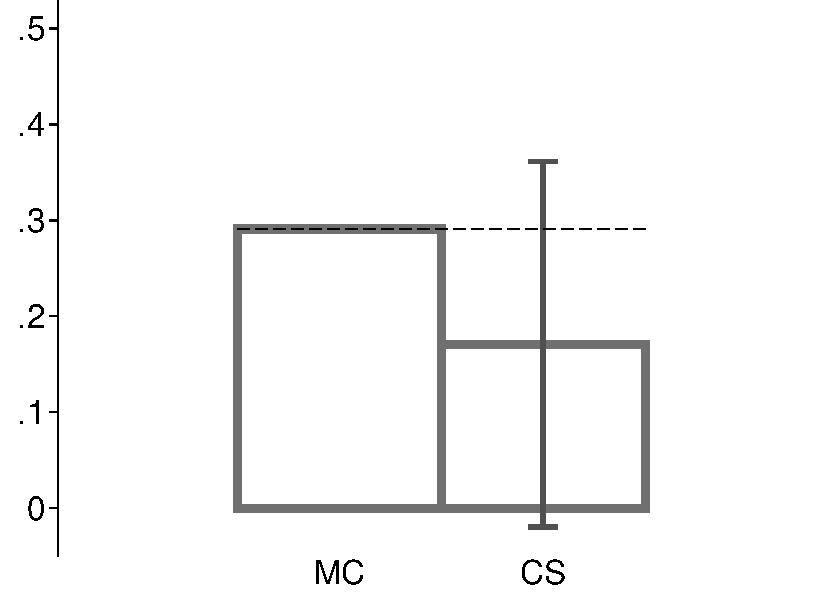
\includegraphics[width=\textwidth]{../figs/confidence_score_ccd_fsr_fsr_religion_study1.pdf}
		\caption{Obama religion}
	\end{subfigure}	
	\hfill
	% First row c
	\begin{subfigure}{.325\textwidth}\centering
		\includegraphics[width=\textwidth]{../figs/confidence_score_ccd_fsr_fsr_illegal_study1.pdf}
		\caption{ACA illegal}
	\end{subfigure}	
	% Second row a
	\begin{subfigure}{.325\textwidth}\centering
		\includegraphics[width=\textwidth]{../figs/confidence_score_ccd_fsr_fsr_death_study1.pdf}
		\caption{ACA death panels}
	\end{subfigure}
	\hfill
	% Second row b
	\begin{subfigure}{.325\textwidth}\centering
		\includegraphics[width=\textwidth]{../figs/confidence_score_ccd_fsr_fsr_increase_study1.pdf}
		\caption{GW causes}
	\end{subfigure}	
	\hfill
	% Second row c
	\begin{subfigure}{.325\textwidth}\centering
		\includegraphics[width=\textwidth]{../figs/confidence_score_ccd_fsr_fsr_science_study1.pdf}
		\caption{GW scientists agree}
	\end{subfigure}	
	% Third row a
	\begin{subfigure}{.325\textwidth}\centering
		\includegraphics[width=\textwidth]{../figs/confidence_score_ccd_fsr_fsr_fraud_study1.pdf}
		\caption{Voter fraud}
	\end{subfigure}
	\hfill
	% Third row b
	\begin{subfigure}{.325\textwidth}\centering
		\includegraphics[width=\textwidth]{../figs/confidence_score_ccd_fsr_fsr_mmr_study1.pdf}
		\caption{MMR vaccine}
	\end{subfigure}	
	\hfill
	% Third row c
	\begin{subfigure}{.325\textwidth}\centering
		\includegraphics[width=\textwidth]{../figs/confidence_score_ccd_fsr_fsr_deficit_study1.pdf}
		\caption{Budget deficit}
	\end{subfigure}	
	\caption*{\footnotesize 
		Bars indicate the predicted percent of correct responses when the correct response is congenial to the party, depending on whether the survey condition is based on Confidence Scoring (CS) or from multiple choice CUD condition (see \cref{tab:conditions} for the descriptions).
		Reconstructed from the estimates from \cref{tab:confidence-scoring-study1-ccd-fsr-fsr}.
		Capped vertical bars indicate 95\% confidence intervals.
	}
	\label{fig:confidence-scoring-study1-ccd-fsr-fsr}
\end{figure}

\begin{figure}[t]
	\caption{Confidence Scoring vs. IMC (MTurk 1)}	
	\centering
	% First row a
	\begin{subfigure}{.325\textwidth}\centering
		\includegraphics[width=\textwidth]{../figs/confidence_score_ccd_imc_14k_birth_study1.pdf}
		\caption{Obama birthplace}
	\end{subfigure}
	\hfill
	% First row b
	\begin{subfigure}{.325\textwidth}\centering
		\includegraphics[width=\textwidth]{../figs/confidence_score_ccd_imc_14k_religion_study1.pdf}
		\caption{Obama religion}
	\end{subfigure}	
	\hfill
	% First row c
	\begin{subfigure}{.325\textwidth}\centering
		\includegraphics[width=\textwidth]{../figs/confidence_score_ccd_imc_14k_illegal_study1.pdf}
		\caption{ACA illegal}
	\end{subfigure}	
	% Second row a
	\begin{subfigure}{.325\textwidth}\centering
		\includegraphics[width=\textwidth]{../figs/confidence_score_ccd_imc_14k_death_study1.pdf}
		\caption{ACA death panels}
	\end{subfigure}
	\hfill
	% Second row b
	\begin{subfigure}{.325\textwidth}\centering
		\includegraphics[width=\textwidth]{../figs/confidence_score_ccd_imc_14k_increase_study1.pdf}
		\caption{GW causes}
	\end{subfigure}	
	\hfill
	% Second row c
	\begin{subfigure}{.325\textwidth}\centering
		\includegraphics[width=\textwidth]{../figs/confidence_score_ccd_imc_14k_science_study1.pdf}
		\caption{GW scientists agree}
	\end{subfigure}	
	% Third row a
	\begin{subfigure}{.325\textwidth}\centering
		\includegraphics[width=\textwidth]{../figs/confidence_score_ccd_imc_14k_fraud_study1.pdf}
		\caption{Voter fraud}
	\end{subfigure}
	\hfill
	% Third row b
	\begin{subfigure}{.325\textwidth}\centering
		\includegraphics[width=\textwidth]{../figs/confidence_score_ccd_imc_14k_mmr_study1.pdf}
		\caption{MMR vaccine}
	\end{subfigure}	
	\hfill
	% Third row c
	\begin{subfigure}{.325\textwidth}\centering
		\includegraphics[width=\textwidth]{../figs/confidence_score_ccd_imc_14k_deficit_study1.pdf}
		\caption{Budget deficit}
	\end{subfigure}	
	\caption*{\footnotesize 
		Bars indicate the predicted percent of correct responses when the correct response is congenial to the party, depending on whether the survey condition is based on Confidence Scoring (CS) or from multiple choice CUD condition (see \cref{tab:conditions} for the descriptions).
		Reconstructed from the estimates from \cref{tab:confidence-scoring-study1-ccd-fsr-fsr}.
		Capped vertical bars indicate 95\% confidence intervals.
	}
	\label{fig:confidence-scoring-study1-ccd-imc-14k}
\end{figure}

\section{Partisan Gaps in Knowledge Across Question Designs}
\begin{center}
	\begin{figure}[ht]
		\centering
		\caption{Partisan Gaps in Knowledge Across Question Designs (Pooled multiple choices)}
		\includegraphics[width=.9\textwidth]{../figs/partisan-gap-by-item-arm-mc-24k.pdf}
		\label{fig:mturk_hk24_mc}
		\caption*{\footnotesize
		The figure shows the estimated partisan gaps in knowledge from the MTurk sample for Study 1 for the four multiple-choice survey conditions (pooling IDA, CUD, FSR, and IMC) and the confidence coding design (CCD). Corresponds to \cref{fig:mturk_hk24}.
            The CCD condition only considers selecting the right answer with complete confidence as evidence that the respondent knows the answer (see \cref{si:mturk2}).
            See \crefrange{tab:confidence-scoring-study1}{tab:confidence-scoring-study1-ccd-14k-imc} in \cref{si:mturk1-ccd} for the regression estimates of the multiple-choice conditions to the confidence coding condition.
		}
	\end{figure}
\end{center}

\clearpage
\section{Item Text for MTurk 1}\label{si:mturk1}
For exposition, we present the conditions using different terms in the main body (see \cref{tab:conditions}). The following shows how our terminologies for conditions map to the MTurk questionnaires.

\begin{itemize}
    \item{\textbf{IP} = \textbf{IDA}} 
    \item{\textbf{RW} = \textbf{CUD}} 
\end{itemize}

\noindent
\textbf{Preface for Different Conditions}

\textbf{RW, IP}\newline
Now here are some questions about what you may know about politics and public affairs.

\textbf{FSR, IMC, CCD}\newline
Now here are some questions about what you may know about politics and public affairs.
We are interested in measuring what people currently know and can recall on their own and are just as interested in what people don't know as in what they do know. So we'd like your agreement to just say ``don't know'' if you don't know the answer—without looking anything up or talking with anyone about it.

\textbf{Item Text}
\textbf{CCD}\newline
Now here are a series of statements. On a scale of 0 to 10, where 0 means definitely false, 10 means definitely true, and 5 is exactly in the middle, how definitely true or false is each statement?

\begin{itemize}
	\item Barack Obama was born in the US (T)
	\item  Barack Obama is a Muslim (F)
	\item  The Affordable Care Act gives illegal immigrants financial help to buy health insurance (F)
	\item  The Affordable Care Act does not create government panels to make decisions about end-of-life care (T)
	\item  Temperatures around the world are increasing because of human activity, like burning coal and gasoline (T)
	\item  Most climate scientists believe that global warming is not occurring (F)
	\item  In the 2016 presidential election, President Trump won the majority of the legally cast votes (F)
	\item  The vaccine for measles, mumps, and rubella (MMR) causes autism in children. (F)
	\item  Since 2012, the annual federal budget deficit has increased. (T)
\end{itemize}

\textbf{Rest of the Conditions, By Item}

\begin{itemize}
\item Obama's Birthplace

\textbf{RW and IP}\newline

According to the Constitution, American presidents must be ``natural-born citizens.''
Some people believe Barack Obama was not born in the United States but was born
in another country. Do you think Barack Obama was born in ...?
\begin{itemize}
	\item The US
	\item Another country
\end{itemize}

\textbf{FSR}\newline
Some people believe Barack Obama was not born in the United States but was born
in another country. Was he born in ...?
\begin{itemize}
	\item The US
	\item Another country
	\item DK (plus DK pref)
\end{itemize}

\textbf{IMC}\newline

Was Barack Obama born in ...?
\begin{itemize}
	\item the US
	\item Another country
	\item DK (plus DK pref)
\end{itemize}

\item Obama Religion\newline
\textbf{RW}\newline

Do you personally believe that Barack Obama is a ...?
\begin{itemize}
	\item Muslim
	\item Christian
\end{itemize}

\textbf{IP}\newline

Most people have a religion. Some people believe Barack Obama is a Muslim. Do you personally believe that Barack Obama is a \ldots?
\begin{itemize}
	\item Muslim
	\item Christian
\end{itemize}

\textbf{FSR}\newline

Some people believe Barack Obama is a Muslim. Is he a \ldots?
\begin{itemize}
	\item Muslim
	\item Christian
	\item DK (+ DK pref)
\end{itemize}

\textbf{IMC}\newline

Is Barack Obama a \ldots?
\begin{itemize}
	\item Muslim
	\item Christian
	\item DK (plus DK pref)
\end{itemize}

\item ACA Illegal\newline
\textbf{RW}\newline

To the best of your knowledge, would you say the Affordable Care Act \ldots?
\begin{itemize}
	\item Gives illegal immigrants financial help to buy health insurance
	\item Does not give illegal immigrants financial help to buy health insurance
\end{itemize}

\textbf{IP}\newline

As you may know, there is currently talk of changing the Affordable Care Act
(ACA), enacted in 2010. Some people believe that the ACA gives illegal immigrants
financial help to buy health insurance. To the best of your knowledge, would you say
the ACA\ldots?
\begin{itemize}
	\item Gives illegal immigrants financial help to buy health insurance
	\item Does not give illegal immigrants financial help to buy health insurance
\end{itemize}

\textbf{FSR}\newline

Some people believe that the Affordable Care Act gives illegal immigrants financial help
to buy health insurance. Does the Affordable Care Act \ldots?
\begin{itemize}
	\item Give illegal immigrants financial help to buy health insurance
	\item Not give illegal immigrants financial help to buy health insurance
	\item DK (+ DK pref)
\end{itemize}

\textbf{IMC}\newline
Does the Affordable Care Act \ldots?
\begin{itemize}
	\item Give illegal immigrants financial help to buy health insurance
	\item Not Give illegal immigrants financial help to buy health insurance
	\item Don't know (+ DK pref)
\end{itemize}

\item ACA—Death Panels\newline
\textbf{RW}\newline
To the best of your knowledge, would you say that the Affordable Care Act \ldots?
\begin{itemize}
	\item Creates government panels to make decisions about end-of-life care
	\item Does not create government panels to make decisions about end-of-life care
\end{itemize}

\textbf{IP}\newline

Some people believe that the Affordable Care Act establishes a government panel to
make decisions about end-of-life care. To the best of your knowledge, would you say
that the Affordable Care Act \ldots?
\begin{itemize}
	\item Creates government panels to make decisions about end-of-life care
	\item Does not create government panels to make decisions about end-of-life care
\end{itemize}

\textbf{FSR}\newline

Some people believe that the Affordable Care Act establishes a government panel to
make decisions about end-of-life care. Does the Affordable Care Act \ldots?
\begin{itemize}
	\item Creates government panels to make decisions about end-of-life care
	\item Does not create government panels to make decisions about end-of-life care
	\item DK (+ DK pref)
\end{itemize}

\textbf{IMC}\newline
Does the Affordable Care Act \ldots?
\begin{itemize}
	\item Creates government panels to make decisions about end-of-life care
	\item Does not create government panels to make decisions about end-of-life care
	\item DK (+ DK pref)
\end{itemize}

\item Global Warming—Happening + Causes\newline
\textbf{RW}\newline
Which of the following best fits your view about this? Are temperatures around the
world \ldots?
\begin{itemize}
	\item Increasing because of the natural variation over time, such as produced by the ice age
	\item Increasing because of human activity, like burning coal and gasoline
	\item Staying about the same as they have been
\end{itemize}

\textbf{IP}\newline
Recently, you may have noticed that global warming has been getting some attention
in the news. Some people believe that temperatures are increasing around the world
because of natural variation over time, such as that produced the ice age. Which of the
following best fits your view about this? Would you say that temperatures around the
world are\ldots?
\begin{itemize}
	\item Increasing because of the natural variation over time, such as produced by the ice age
	\item Increasing because of human activity, like burning coal and gasoline
	\item Staying about the same as they have been
\end{itemize}

\textbf{FSR}\newline

Some people believe that temperatures are increasing around the world because of
natural variation over time, such as produced the ice age. Are temperatures around
the world \ldots?
\begin{itemize}
	\item Increasing because of the natural variation over time, such as produced by the ice age
	\item Increasing because of human activity, like burning coal and gasoline
	\item Staying about the same as they have been
	\item DK (+ DK pref)
\end{itemize}

\textbf{IMC}\newline
Are temperatures around the world \ldots?
\begin{itemize}
	\item Increasing because of natural variation over time, such as produced by the ice age
	\item Increasing because human activity, like burning coal and gasoline
	\item Staying about the same as they have been
	\item DK (+ DK pref)
\end{itemize}

\item GW—Scientist Agreement\newline
\textbf{RW}\newline
Just your impression, which one of the following statements do you think is most
accurate?
\begin{itemize}
	\item Most climate scientists believe that global warming is occurring.
	\item Most climate scientists believe that global warming is not occurring.
	\item Climate scientists are about equally divided about whether global warming is occurring or not
\end{itemize}

\textbf{IP}\newline
As you may know, the term ``global warming'' refers to the claim that temperatures
have been increasing around the world. Some people believe that most climate
scientists believe that global warming is not occurring. Just your impression, which
one of the following statements do you think is most accurate?
\begin{itemize}
	\item Most climate scientists believe that global warming is occurring.
	\item Most climate scientists believe that global warming is not occurring.
	\item Climate scientists are about equally divided about whether global warming is occurring or not
\end{itemize}
\textbf{FSR}\newline
Some people believe that most climate scientists believe that global warming is not
occurring. Which one of the following statements is most accurate?
\begin{itemize}
	\item Most climate scientists believe that global warming is occurring.
	\item Most climate scientists believe that global warming is not occurring.
	\item Climate scientists are about equally divided about whether global warming is occurring or not
	\item DK (+ DK pref)
\end{itemize}

\textbf{IMC}\newline
Which one of the following statements is most accurate?
\begin{itemize}
	\item Most climate scientists believe that global warming is occurring.
	\item Most climate scientists believe that global warming is NOT occurring.
	\item Climate scientists are about equally divided about whether global warming is occurring or not
	\item DK (+ DK pref)
\end{itemize}

\item Voter Fraud\newline
\textbf{RW}\newline
As you may know, President Trump has said that several million people voted
illegally in the 2016 presidential election and that he won the majority of the legally
cast votes. Do you believe that President Trump \ldots?
\begin{itemize}
	\item Won the majority of the legally cast votes
	\item Did not win the majority of the legally cast votes
\end{itemize}

\textbf{IP}\newline
As you may know, not everyone living in the US has the legal right to vote. President
Trump has said that several million people voted illegally in the 2016 presidential
election and that he won the majority of the legally cast votes. Do think that
President Trump \ldots?
\begin{itemize}
	\item Won the majority of the legally cast votes
	\item Did not win the majority of the legally cast votes
\end{itemize}

\textbf{FSR}\newline
As you may know, President Trump has said that several million people voted
illegally in the 2016 presidential election and that he won the majority of the legally
cast votes. Did President Trump \ldots?
\begin{itemize}
	\item Won the majority of the legally cast votes
	\item Did not win the majority of the legally cast votes
	\item DK (+ DK pref)
\end{itemize}

\textbf{IMC}\newline
In the 2016 presidential election, did President Trump \ldots?
\begin{itemize}
	\item Won the majority of the legally cast votes
	\item Did not win the majority of the legally cast votes
	\item DK (+ DK pref)
\end{itemize}

\item Vaccines\newline
\textbf{RW}\newline
From what you have read or heard, do you personally think that the vaccine for
Measles, Mumps, and Rubella (MMR):
\begin{itemize}
	\item Causes autism in children
	\item Does not cause autism in children
\end{itemize}

\textbf{IP}\newline
As you may know, most children receive the vaccine for Measles, Mumps, and
Rubella (MMR). Some people believe that the MMR vaccine causes autism in
children. From what you have read or heard, do you personally think that the MMR
vaccine:
\begin{itemize}
	\item Causes autism in children
	\item Does not cause autism in children
\end{itemize}

\textbf{FSR}\newline
Some people believe that the vaccine for Measles, Mumps, and Rubella (MMR)
causes autism in children. Does the MMR vaccine \ldots?
\begin{itemize}
	\item Cause autism in children
	\item Not cause autism in children.
	\item DK (+ DK pref)
\end{itemize}

\textbf{IMC}\newline
Does the vaccine for Measles, Mumps, and Rubella (MMR) \ldots?
\begin{itemize}
	\item Cause autism in children
	\item Not cause autism in children.
	\item DK (+ DK pref)
\end{itemize}

\item Obama—Budget Deficit\newline
\textbf{RW}\newline
As you may know, the federal government runs a deficit when it spends more than it
takes in. Since 2012, would you say that the annual federal budget deficit has \ldots
\begin{itemize}
	\item Increased
	\item Stayed about the same
	\item Decreased
\end{itemize}

\textbf{IP}\newline
As you may know, the federal government runs a deficit when it spends more than it
takes in. Since 2012, with the Republicans having the majority in the U.S. House of
Representatives, would you say that the annual federal budget deficit has \ldots
\begin{itemize}
	\item Increased
	\item Stayed about the same
	\item Decreased
\end{itemize}

\textbf{FSR}\newline
Since 2012, with the Republicans having the majority in the U.S. House of
Representatives,
\begin{itemize}
	\item has the annual federal budget deficit \ldots.
	\item Increased
	\item Stayed about the same
	\item Decreased
	\item DK (+ DK pref)
\end{itemize}

\textbf{IMC}\newline

Since 2012, has the annual federal budget deficit \ldots
\begin{itemize}
	\item Increased
	\item Stayed about the same
	\item Decreased
	\item DK (+ DK pref)
\end{itemize}
\end{itemize}

\newpage

\clearpage
\section{Criterion Variables}\label{si:mturk1_criteria}
\begin{itemize}

    \item Political Interest: On a scale from 0 to 10, where 0 is not at all, 10 is passionately, and 5 is exactly in the middle, how interested would you say you generally are in politics and public affairs?

    \item Vote: Again on a scale from 0 to 10, where now 0 means certain not to vote, 10 means certain to vote, and 5 is exactly in the middle, how likely would you say you are to vote in the next Congressional elections?

    \item What's the highest level of education you have obtained? No High School Diploma, High School Diploma or Equivalent, Some College, Four-year College Graduate, Post-graduate Degree
\end{itemize}

\clearpage
\section{Item Text for MTurk 2}\label{si:mturk2}

The second Amazon MTurk survey was fielded in April 2017 and had 1,059 participants. In this survey, we made use of new questions and probes to examine the effect of question design on (partisan) knowledge. We asked the participants four questions about the Affordable Care Act (2), the effect of greenhouse gases (1), and Donald Trump's recent executive order on immigration (1).

One-half of the survey respondents got a conventional closed-ended item with five options including the opportunity to mark Don’t know. The other half of the respondents had to assess the truth of statements on a scale from definitely false (0) to definitely true (10).

\begin{description}
\item[1.] Does the Affordable Care Act ...?
  \begin{itemize}
    \item  CE: Provide coverage for people who are currently in the country illegally, Replace private health insurance with a ``single-payer system'', \textbf{Increase the Medicare payroll tax for upper-income Americans}, Reimburse routine mammograms only for women older than 50, Don’t know (5)
    \item  Scale: Rating each response option above from definitely false (0) to definitely true (10). Don't know was not included. See Figure \ref{fig:aca1}.
    \end{itemize}
    \item[2.] Are greenhouse gases ...?
  \begin{itemize}
  \item CE: A cause of respiratory problems, A cause of lung cancer, Damaging the ozone layer, \textbf{A cause of rising sea levels}, or Don't know
  \item Scale: Rating each response option above from definitely false (0) to definitely true (10). Don't know was not included. See Figure \ref{fig:gg1}.
    \end{itemize}
  \item[3.] And does the Affordable Care Act ...?
    \begin{itemize}
  \item CE: Create government panels to make end-of-life decisions for people on Medicare, Replace Medicare with a ``public option'', \textbf{Limit future increases in payments to Medicare providers}, Cut benefits to existing Medicare patients, Don’t know
  \item Scale: Rating each response option above from definitely false (0) to definitely true (10). Don't know was not included. See Figure \ref{fig:aca2}.
    \end{itemize}
        \item[4.] Does President Trump’s most recent executive order on immigration ...?
  \begin{itemize}
  \item  CE: Subject immigrants living in the U.S. illegally to deportation, Strip immigrants from countries supporting terrorism of their green cards, Strip immigrants from several Muslim-majority countries of their green cards, \textbf{Temporarily ban immigrants from several majority-Muslim countries}, Don’t know
    \item  Scale: Rating each response option above from definitely false (0) to definitely true (10). Don't know was not included. See Figure \ref{fig:eo1}.
    \end{itemize}
    \end{description}

If the close-ended questions 3 and 4 were not answered with Don’t know the respondents received one of two follow-up questions:
\begin{itemize}
\item OE: What made you choose that response?
 \item CE: What made you choose that response? I asked someone I know, I looked it up, I've read, seen, or heard that, It makes me feel good to think that, It makes sense, in view of other things I know, I just thought I’d take a shot
\end{itemize}

\begin{center}
	\begin{figure}[H]
		\centering
		\caption{Affordable Care Act 1 Scale Question}
		\includegraphics[width=\textwidth]{../figs/hk_aca1.png}
		\label{fig:aca1}
		\caption*{\footnotesize }
	\end{figure}
\end{center}


\begin{center}
	\begin{figure}[H]
		\centering
		\caption{Greenhouse Gases Scale Question}
		\includegraphics[width=\textwidth]{../figs/hk_gg1.png}
		\label{fig:gg1}
		\caption*{\footnotesize }
	\end{figure}
\end{center}


\begin{center}
	\begin{figure}[H]
		\centering
		\caption{Affordable Care Act 2 Scale Question}
		\includegraphics[width=\textwidth]{../figs/hk_aca2.png}
		\label{fig:aca2}
		\caption*{\footnotesize }
	\end{figure}
\end{center}


\begin{center}
	\begin{figure}[H]
		\centering
		\caption{Executive Order Scale Question}
		\includegraphics[width=\textwidth]{../figs/hk_eo1.png}
		\label{fig:eo1}
		\caption*{\footnotesize }
	\end{figure}
\end{center}

\clearpage
\section{Proportion Correct across Questions}

Table \ref{tab:prop_correct} shows the proportion of correct answers across the Affordable Care Act questions (ACA and ACA2), the Greenhouse Gas question, and the question about Donald Trump's executive order. We report the proportion correct for closed questions in the multiple-choice format and the relative scoring at the thresholds of 8 and 10. For the relative scoring to code an answer as correct the confidence for the correct answer had to be 8 (or 10), the scoring had to be the maximum number given, it had to be unique, and incorrect answers were not allowed to be scored higher than 2 (or 0). 

\input{tabs/tab_prop_correct.tex}

\clearpage
\section{Less Stringent Coding Criteria for CCD}
\label{si_alternate_coding}

\begin{center}
	\begin{figure}[ht]
		\centering
            \caption{Robustness check for Confidence Scoring and Knowledge Gaps: MTurk 1}
		\includegraphics[width=.9\textwidth]{../figs/partisan-gap-by-item-arm-14k-24k-greaterthan7.pdf}
		\label{fig:mturk_hk24_greaterthan7}
		\caption*{\footnotesize
		The figure shows the estimated partisan gaps in knowledge from the MTurk sample for Study 1 for two different survey conditions. The CCD condition only considers selecting the right answer with confidence larger than 7 as evidence that the respondent knows the answer (see \cref{si:mturk2}). Corresponds to \cref{fig:mturk_hk24}, the difference here is that the analysis implements a relative scoring threshold of 8. See \cref{tab:tab6_robustness} for the analogous table for Study 3: MTurk 2 Results.
		}
	\end{figure}
\end{center}


\input{tabs/tab6_replication_threshold8.tex}


\end{document}